\documentclass[conference]{IEEEtran}

\linespread{1.2}
\usepackage[margin = 1.25 in]{geometry}
\usepackage{wrapfig}
\usepackage{amsfonts}
\usepackage[utf8]{inputenc}
\usepackage[T1]{fontenc}
\usepackage{graphicx}
\usepackage[english]{babel}
\usepackage[algoruled]{algorithm2e}

\renewcommand{\theequation}{\thesubsection.\arabic{equation}}
\DeclareGraphicsExtensions{.pdf,.png,.jpg, .gif}



\usepackage[english]{babel}
\usepackage{mathtools}

%\usepackage[OT2,T1]{fontenc}
%\DeclareSymbolFont{cyrletters}{OT2}{wncyr}{m}{n}
%\DeclareMathSymbol{\sha}{\mathalpha}{cyrletters}{"58}

\DeclareFontFamily{U}{wncy}{}
\DeclareFontShape{U}{wncy}{m}{n}{<->wncyr10}{}
\DeclareSymbolFont{mcy}{U}{wncy}{m}{n}
\DeclareMathSymbol{\Sh}{\mathord}{mcy}{"58} 
\DeclareMathOperator*{\argmin}{arg\,min}

\newcounter{eqn}
\renewcommand*{\theeqn}{\alph{eqn})}
\newcommand{\num}{\refstepcounter{eqn}\text{\theeqn}\;}

\makeatother
\newcommand{\vectornorm}[1]{\left|\left|#1\right|\right|}
\newcommand*\conjugate[1]{\bar{#1}}

\newtheorem{thm}{Theorem}
\newtheorem{defn}{Definition}
 %\theoremstyle{plain}
  \newtheorem{theorem}{Theorem}[section]
  \newtheorem{corollary}[theorem]{Corollary}
  \newtheorem{proposition}[theorem]{Proposition}
  \newtheorem{lemma}[theorem]{Lemma}
\newtheorem{example}[theorem]{Example}
  \newtheorem{definition}[theorem]{Definition}
  \newtheorem{conj}[theorem]{Conjecture}
 \newtheorem{condition}{Condition}
 \newtheorem{remark}[theorem]{Remark}

\newcommand{\supp}{\operatorname{supp}} 
\newcommand{\vc}[1]{{\mathbf{ #1}}}
\newcommand{\tn}{\widetilde{\nabla}_{n} }
\newcommand{\Z}{{\mathbb{Z}}}
\newcommand{\re}{{\mathbb{R}}}
\newcommand{\II}{{\mathbb{I}}}
\newcommand{\ep}{{\mathbb{E}}}
\newcommand{\pr}{{\mathbb{P}}}
\newcommand{\FF}{{\mathcal{F}}}
\newcommand{\TT}{{\mathcal{T}}}
\newcommand{\phin}{\phig{n}}
\newcommand{\phig}[1]{\phi^{(#1)}}
\newcommand{\ol}[1]{\overline{#1}}
\newcommand{\eff}{{\rm eff}}
\newcommand{\suc}{{\rm suc}}
\newcommand{\tends}{\rightarrow \infty}
\newcommand{\setS}{{\mathcal{S}}}
\newcommand{\setP}{{\mathcal{P}}}
\newcommand{\setX}{{\mathcal{X}}}
\newcommand{\nec}{{\rm nec}}
\newcommand{\bd}{{\rm bd}}
\begin{document}

\title{End of year report 2014}
\author{Tom Kealy}

\bibliographystyle{abbrv}

\maketitle

\section{Introduction}
Despite the ubiquity, capacity and apparent efficacy, modern communication systems are wasteful, inefficient and in need of reform. Most of the bits of data collected by our sensing systems are unessential, and only serve to necessitate data compression wasting computation time before transmission. For example, people regularly use a camera with a resolution of several megapixels only to upload a file of a few kilobytes to Facebook. Devices are unable to make dynamic decisions about how to transmit this data, leading to both spectral exhaustion on some frequencies whilst much of the available radio spectrum lies fallow. 

This project addresses these issues, by reviewing a novel acquisition and decompression framework for data: a way in which we need only sense the most informative bits of data. This framework is then applied to the problem of sensing spectral opportunities dynamically, to make better use of available spectrum. 

The key uniting both these applications is that data and spectra are \textit{sparse}: that is they have a representations which are 'smaller' than their respective dimension. For example, images and audio can be compressed into file formats much smaller than when initially recorded (compare the relative sizes of bitmap and JPEG images).

The sole focus of this research is to use the sparsity of the spectrum to uncover transmission opportunities, allowing better use of spectrum more generally. 

We are motivated by the need to send more data over wireless networks, whilst at the same time having a constrained frequency set over which to transmit this information. This issue could be alleviated by users dynamically allocating spectrum on a per-transmission basis: without the ability to gain knowledge of spectral conditions this can never become a reality however. 

The requirement for increasing bandwidth isn't just a pressing issue for today: in the next decade it is forecast that network operators will need to provide for three-orders of magnitude (1000 times) more capacity. Demand is continually outstripping supply - motivated by the ubiquity of smart-phones, and the consumers appetites for media. 

At the same time as this demand for ever more data, there is an increasing scarcity of radio spectrum over which to transmit. New frequencies are rarely cleared for commercial purposes, and when they are they go for high prices.  A decade ago the UK auction for 3g spectrum licenses raised an estimated £22.4 billion \cite{Ukmobil} for the UK treasury, indicating the seriousness of the market players requirements for new spectrum. The recent 4g spectrum auction raised £2.3 billion \cite{BBC News}- with initial networks being rolled out by the end of 2013.

\begin{figure*}[h]
\centering
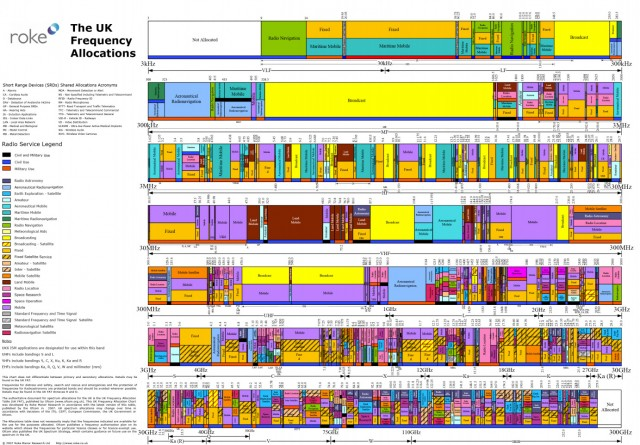
\includegraphics[height = 7 cm]{uk-spectrum-allocation-chart1-640x445.jpg}
\caption{A digram of current Spectral allocation \cite{Strategy2013}}
\label{spectrumalloc}
\end{figure*}

However, a closer inspection of the frequency allocation suggests this scarcity is artificial, it's more a product of regulatory oversight over time. As the constraints on spectrum requirement became more complex, so did the solutions to that problem - at the cost of leaving much of the spectrum idle for most of the time. 

For example: much of the spectrum is allocated to TV broadcast, radio broadcast and mobile. However, if we look closer, the allocations aren't even for specific companies - they're simply categories. Within these, OFCOM may have many licensees within each category.

Also interesting to note is how much frequency the Government allocates to itself (the red bar underneath the blocks indicates Government use). Compare this to the actual utilisation of spectrum: much of it is not used at all. Figure \ref{frequtil} shows a snapshot of frequency utilisation in three diverse locations in the UK over te radio specturm, note that many frequencies are not utilised (coloured blue) whilst others have significant activity (coloured yellow). Note that the plot for Southwark (central London) is barely different from Braddock - a rural area. 

\begin{figure*}[h]
\centering
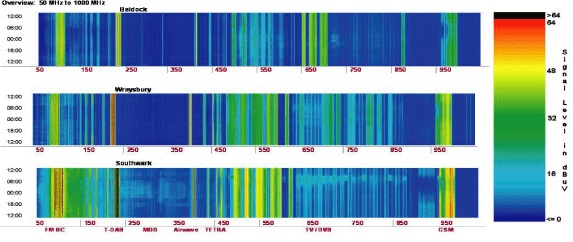
\includegraphics[height = 7 cm, width=0.5\textwidth]{cr2.jpg}
\caption{A snapshot of frequency utilisation in various areas: many frequencies are not used at all, whilst there is significant activity on others \cite{Burbidge2007}}
\label{frequtil}
\end{figure*}

How do we then go about solving this issue - how can we obtain the most significant bits of information from our sensing mechanism, whilst obviating the need to compress the data once we are done? How do we dynamically assign spectrum? The work of Candes, Tao \cite{Candes2006} and Donoho \cite{Donoho2006}, has shown that instead of measuring the information we require directly (and then compressing it), we can measure 'holographic' and non-linear random projections between our measurement space and the space where our data is sparse. This requires only the knowledge that the signal is compressible via some transform - both the acquisition protocol and the reconstruction algorithm are agnostic to the type of signal. What is surprising is that the sampling kernels are fixed independently of the signal, are non-adaptive and these projections are sufficient to reconstruct the signal - as if we had an Oracle to tell us where the non-zero components of our signal are. 

This work has had a large impact in medical imaging since it's inception: for example, it's now possible to take an image of a patient's heart within a single breath, as well as dynamic imaging of the heart (\cite{Donoho} figures 7 and 9).

Modern digital signal processing techniques (such as modulation techniques) are far more spectrally efficient than their historic analogue counterparts, which has in part contributed to the spectrum crisis. All this is changing though: from the beginning of 2013 all TV in the UK will transmitted digitally. Historically, television in the UK was broadcast using analogue signals requiring 32 multiplexes. Digital TV requires 6 multiplexes, on the other hand. 

This freeing up of TV frequencies represents an opportunity: these frequencies have good propagation characteristics (they suffer less with free space path loss relative to higher frequencies), whilst sill providing good bandwidth for data transmission. These TV frequencies are being opened up to civilian and  commercial users: spectral holes will be able to be exploited opportunistically by devices, so long as they don't interfere with the reception of TV. Historically, this is the single largest gift of new spectrum, and because there is no requirement for licensing this spectrum is free.

\begin{wrapfigure}{r}{0.5\textwidth}
\centering
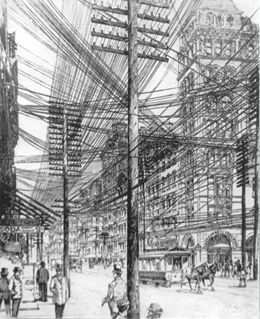
\includegraphics[width=0.48\textwidth, height = 7cm]{cablesnewyork.jpg}
\caption{A picture of early 20th century New York: Bandwidth has always been an issue}
\label{newyork}
\end{wrapfigure}

As with all technological innovations, this will not only improve existing infrastructure but also new classes of devices to transmit, for instance; applications such as passive sensor networks) which only need spectrum intermittently to transmit monitoring results), inter-vehicle communication for real time traffic monitoring and wireless internet at broadband data rates have all been proposed.

Despite all of this hype, dynamic spectrum access won't become a reality unless spectral holes can be robustly detected. The requirement that secondary users exploit the new spectrum politely, without interference to primary user makes spectrum sensing essential to TV white-space (TVWS) technologies. The realisation of any Cognitive Radio standard (such as IEEE 802.22), requires the co-existence of primary (TV users) and secondary (everybody else who wants to use TVWS spectrum) users of the frequency spectrum to ensure proper interference mitigation and appropriate network behaviour. 

Users of TVWS (Cognitive Radios) must sense whether spectrum is available, and must be able to detect very weak primary user signals. Furthermore they must sense over a wide bandwidth (due to the amount of TVWS spectrum proposed), which challenges traditional Nyquist sampling techniques, because the sampling rates required are not technically feasible with current RF or Analogue-to-Digital conversion technology.

Sensing should enable devices to detect the presence of TV signals in a band and provide smart and adaptive (and possibly distributed) solutions to band identification.

Spectrum sensing should involve:

\begin{enumerate}
\item Sensing to detect white spaces.
\item Co-existence with similar devices.
\item Frequency monitoring of other devices.
\item Interference management. 
\item Spectrum mobility and transmission power control when needed.
\end{enumerate}

As described earlier, the available spectrum is highly underutilised, and can be thought of as a collection of narrowband transmissions over a wideband channel. As such, the spectrum we're sensing is sparse. This makes it an ideal candidate for sparse recovery techniques such as Compressive Sensing.  

The structure of the report is as follows: first a few methods for sensing narrowband signals (i.e. channels where the frequency response is approximately flat, and where the bandwidth is smaller than the coherence bandwidth of the channel) are discussed and the limitations of these are highlighted for the problem of sensing spectrum for Cognitive Radios. Then (more appropriate) wideband sensing techniques are discussed. 

Compressive Sensing, and Group Testing are then introduced and it is argued that they offer appropriate solutions to the sensing problems for cognitive radios. Sampling schemes married to these reconstruction algorithms are discussed. 

Finally the results and simulations performed over the time-frame of the project are discussed, with reference to further work. 

\section{Narrowband Spectrum Sensing}

The problem of spectrum sensing is to decide whether a particular band is available, or not \cite{Y}. That is, we wish to discriminate between the following two hypotheses:

\begin{equation}
H_{0}: y\left[n\right] = w\left[n\right] \text{, n} =  1 \ldots N 
\end{equation}
\label{h1}

\begin{equation}
H_{1}: y\left[n \right] = x\left[n\right] + w\left[n\right] \text{, n} =  1 \ldots N 
\end{equation}
\label{h2}

Where \(x\) is the primary users signal, having a specific structure which stems from modern coding and modulation techniques, \(w\) is additive white Gaussian noise and \(y\) is the received signal.

To decide whether the observations \(\textbf{y}\) were generated under \(\textit{H}_{0}\) or \(\textit{H}_{1}\) is accomplished by forming a test statistic \(\Gamma\left(y\right)\) and then comparing this statistic with a predefined threshold \(\lambda\). Both classical methods, where the hypotheses are assumed to be deterministically true and the goal is to minimise the false detection probability, and Bayesian methods, where it is assumed that the source selects the true hypothesis at random according to some prior probabilities, agree that the test statistic should be likelihood ratio:

\begin{equation}
\Gamma\left(\textbf{y}\right) = \frac{p\left(\textbf{y}\mid H_0\right)}{p\left(\textbf{y}\mid H_1\right)}
\end{equation}

The performance of a detector is quantified in terms of the probability of detection

\begin{equation}
P_{D} = Pr\left( \Gamma\left(\textbf{y}\right) > \lambda \mid H_1\right)
\end{equation}

and the probability of false alarm 

\begin{equation}
P_{FA} = Pr\left( \Gamma\left(\textbf{y}\right) > \lambda \mid H_0\right)
\end{equation}

By varying \(\lambda\) the operating point of a detector can be chosen anywhere along its receiver operating characteristics curve.

There are several proposed spectrum sensing methods that enable cognitive radios identify bands and perform dynamic frequency selection. Some of the common (narrowband) spectrum sensing techniques are described below.

\subsubsection{Energy Detection}
This is a common method for the detection of unknown signals in noise, due to low computational and implementation complexity. This method is quite generic as receivers need no knowledge of the primary users signal. 

A typical method would be a bandpass filter with a centre frequency \(f_{s}\) and a bandwidth \(W\). This is followed by a squaring device to measure the received energy and an integrator to determine the observation interval. Finally the output of the integrator is compared with a threshold to determine the presence of a signal. This threshold is determined based upon the noise variance of the channel. I.e. we have a decision metric of the following form:

\begin{equation}
M = \sum_{n=0}^N |y\left[n\right]|^2
\end{equation}

Assuming that the signal is a zero mean AWGN variable as well, we can derive expressions for the metric, the detection probability and the false alarm probability:

\begin{equation}
 M =
  \begin{cases}
   \frac{\sigma_w^2}{2} & H_0 \\
   \frac{\sigma_w^2 + \sigma_s^2}{2} & H_1
  \end{cases}
\end{equation}

\begin{equation}
P_D = 1 - \Gamma\left(1, \frac{\lambda}{1 + \frac{ \sigma_2^2 }{ \sigma_w^2 } } \right)
\end{equation}

\begin{equation}
P_FA = 1 - \Gamma\left(1, \frac{\lambda}{\sigma_w^2} \right)
\end{equation}

Where \( \Gamma\left(1,x\right)\) is the incomplete gamma function. From these equations it's clear to see that the performance of energy detection based sensing faces challenges at low SNR values. See (REF) figure 3 for curves quantifying the performance. Also energy detectors perform poorly under extreme fading conditions as they are unable to distinguish primary users and noise. Further this type of detector is not efficient at detecting spread spectrum signals. 

Similarly because the threshold used to make the decision is based on the noise variance \(\sigma_w^2\), any error in the noise power estimation can cause significant performance loss. Various algorithms have been proposed to estimate this variance adaptively. See \cite{Yucek2009} for more details.

\subsubsection{Cyclostationary Feature Detection}
Because the signals used in practical communication systems contain distinctive features that can be exploited for detection, it is possible to achieve a detection performance which substantially surpasses the energy detector. This is in contrast to the predictions of information theory where maximum entropy signals will be statistically white and Gaussian (if this were the case, then we could do no better than the energy detector). More importantly, known signal features can be exploited to estimate unknown parameters such as noise power. 

Examples of well known patterns include pilot signals and spreading sequences. Other examples include preambles and midambles: known sequences transmitted before and in the middle of each slot, respectively. Others include redundancy added by coding, modulation and burst formatting used by the transmitter. 

This method exploits cyclostationary features of received signals: man made periodicity in the signal (for example symbol rate, chip rate, cyclic prefix etc) or its statistics - mean, autocorrelation. A cyclic correlation function is used instead of PSD (or autocorrelation sequence) for detecting signals present in a given spectrum. This is able to differentiate noise from primary users signals since noise is wide-sense stationary with no correlation but modulated signals are cyclostationary due to the redundancy of signal correlations. 

For clarity, the random processes encountered by a cognitive radio will have a period in both expectation and autocorrelation:

\begin{equation}
\mathbb{E}\left(t\right) = \mathbb{E}\left(t + mT\right) = \mathbb{E}\left[x\left(t\right)\right]
\end{equation}

\begin{equation}
\mathbb{R}\left(t, \tau\right) = \mathbb{R}\left(t + mT, \tau\right) = \mathbb{E}\left[x\left(t\right)\conjugate{x\left(t_+\tau\right)}\right]
\end{equation}

where \(t\) is time, \(\tau\) is the autocorrelation lag, \(x\left(t\right)\) is the random process we are considering and \(m\) is an integer. 

Due to the periodicity of the autocorrelation, it can be expressed as a Fourier series over integer multiples of the fundamental frequency in the signal as well as integer multiples of sums and differences of this frequency:
%
\begin{equation}
\mathbb{R}\left(t, \tau\right) = \sum_{\alpha} r\left(\alpha, \tau\right) e^{2\pi j \alpha t}  
\end{equation}
\label{cyclic-covarience}
%
with Fourier coefficients:
%
\begin{equation}
r\left(\alpha, \tau\right) = \frac{1}{T} \int_{T} x\left(t+\frac{\tau}{2}\right)\conjugate{x\left(t+\frac{\tau}{2}\right)} e^{-2\pi j \alpha t} dt
\end{equation}
%
where \(\alpha\) is the cyclic frequency

From this we can define the Cyclic Power Spectrum of the signal:

\begin{equation}
S\left(f\right) = \int_{-\infty}^{\infty} r\left(\alpha, \tau\right) e^{-2 \pi j f \tau} d\tau
\end{equation}

For a fixed lag \(\tau\), \ref{cyclic-covarience} can be re-written as:
%
\begin{equation}
R_{xx}\left(t, \tau \right) = R_{xx}\left(\tau\right) + \sum_{\alpha} r\left(\alpha, \tau\right) e^{2\pi j \alpha t}  
\end{equation}
%
i.e. a part dependent on the lag only (the cyclic frequency is zero), and a part which is a periodic function of time. 

Under both hypotheses, (\ref{h1}, \ref{h2}), the continuous portion of the signal exists, but the cyclo-stationary portion only exists under \ref{h2} when \(\alpha \neq 0\). Thus we only need to test for the presence of a cyclo-statrionary component. 

To this end re-write the hypotheses as:

\begin{equation}
H_{0}: y\left[n\right] = S_{w}^\alpha \left[n\right] \text{, n} =  1 \ldots N 
\end{equation}
\label{c1}

\begin{equation}
H_{1}: y\left[n \right] = S_{x}^{\alpha} \left[n\right] + S_{w}^{\alpha} \left[n\right] \text{, n} =  1 \ldots N 
\end{equation}
\label{c2}

where \(S_{x}^{\alpha}\) is the CPS of white noise which is zero for \(\alpha \neq 0 \).  Using the test statistic:

\begin{equation}
\chi = \sum_{\alpha \neq 0} \sum_{n} S_{x}^{\alpha} \conjugate{S_{x}^{\alpha}}
\end{equation}

we can formulate the cyclo-stationary detector as:

\begin{equation}
 d =
  \begin{cases}
   0 & \chi < \lambda  \\
   1 & \chi \geq \lambda
  \end{cases}
\end{equation}

where \(\lambda\) is some pre-determined threshold \cite{Ghozzi2006}. 

\subsubsection{Matched Filtering}
If all the probability distributions and parameters  - noise variance, signal variance, channel coefficients etc - are known under both hypotheses, and the signal to be detected is perfectly known then the optimal test statistic is a matched filter.

A matched filter is the convolution of a test signal with a template signal (or window) and detects the presence of the template in the unknown signal (as the convolution measures the overlap of two signals).

For example: for a given TV signal, \(r\left(t\right)\) defined over \(0 \leq t \leq T\) the corresponding matched filter is \(h\left(t\right) = r\left(T - t\right)\). 

A test statistic can be formed by sampling the output of the filter every \(nT\) seconds and choosing \ref{h1} if the statistic is below some threshold and \ref{h2} otherwise.

When compared to other methods, matched filtering takes a shorter time to achieve a threshold probability of false alarm. However, matched filtering requires that radios demodulate received signals, and so requires perfect knowledge of primary users signalling features. Matched filtering also requires a prohibitively large power consumption, as various algorithms need to be executed for detection.

\subsubsection{Limitations}
The methods described above, are appropriate for sensing whether a single channel is available for transmission, based upon the result of measurements of that channel. However, Cognitive Radios aim to exploit spectral holes in a wide band spectrum (i.e. a channel whose frequency response is not flat over the bandwidth) and will usually have to make a decision regarding transmission from measurements from this type of channel.

There are two proposed approaches to this: Multiband sensing and Compressive Sensing. Multiband sensing splits the wideband spectrum into a number of independent (not necessarily contiguous) sub-channels (whose frequency response is flat), and performs the hypothesis test for each sub-channel. However, in practice, there are correlations across sub-channels that this method fails to address. For example, digital TV signals are transmitted as spread spectrum signals so that primary user occupancy is correlated across channels. A related issue is that noise variance could be unknown but correlated across bands. Binary hypothesis testing then fails in this case, needing to be replaced by composite hypothesis tests which grow exponentially with the number of sub-channels. Such problems are typically non-convex and require prohibitively complex detectors.

\section{Wideband Spectrum Sensing}
This section presents a new method of sensing sparse signals, and its application to the problem of sensing over wideband spectra in Cognitive Radios. Initially we introduce Classical Sensing and then give an overview of both Compressive Sensing and Group Testing. Finally, we discuss some sub-Nyquist sampling techniques.

\begin{figure*}[h]
\centering
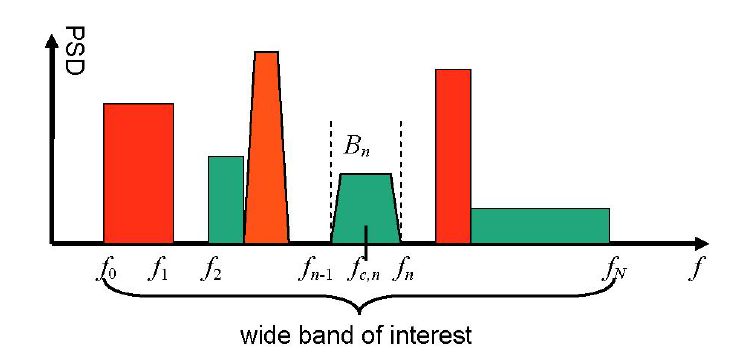
\includegraphics[height = 7 cm]{bands.png}
\caption{A digram of the Spectrum Sensing model \cite{Tian}}
\label{widebandspectra}
\end{figure*}

\subsection{Classical Sensing}
Classically, for perfect signal reconstruction, we must sample a signal such that the sampling rate must be at least twice the maximum frequency in the bandlimited signal. The continuous time signal can then be recovered using an appropriate reconstruction filter (e.g. a sinc filter). For example, we can represent a sampled continuous signal as a multiplication of the signal with a train of Dirac delta functions at multiples of the sampling period T.
%
\begin{equation}
x\left(nT\right) = \Sh\left(t-nT\right)x\left(t\right)
\end{equation}
%
where
%
\begin{equation}
\Sh\left(t-nT\right) = \sum_{k=-\infty}^{\infty} \delta\left(t - kT\right)
\end{equation}

Working the frequency domain, this multiplication becomes convolution (which is equivalent to shifting):

\begin{equation}
\hat{X}_{s}\left(f\right) = \sum_{k=-\infty}^\infty x\left(t - kT\right)
\end{equation}

Thus if the spectrum of the frequency is supported on the interval \(\left(-B, B\right)\) then sampling at intervals \(\frac{1}{2B}\) will contain enough information to reconstruct the signal \(x(\left(t\right)\). Multiplying the spectrum by a rectangle function (low-pass filtering), to remove any images caused by the periodicity of the function, and the signal \(x(\left(t\right)\) can be reconstructed from its samples:

\begin{equation}
x\left(t\right) = \sum_{n=-\infty}^\infty x\left(nT\right) sinc\left(\frac{t_nT}{T}\right)
\end{equation}

\subsection{Compressed Sensing}

However, in practice many signals encountered 'in the wild' can be fully specified by much fewer bits than required by the sampling theorem above. For example, image compression algorithms can reduce the size of a stored image to about 1\% of the size required by Nyquist sampling. If the reconstruction algorithm is able to reconstruct the image from this small amount of data, this raises the question: why collect all the data in the first place, when most of the information can be thrown away? Why not directly measure the part that will not end up being thrown away?

Compressed Sensing considers situations where the signal is \textit{undersampled} i.e. situations in which the number of samples is much smaller than the dimension of the signal (or the number of samples required by classical sampling theory). This is equivalent to a system of linear equations which is under-determined.  That is, this is a method of measuring the informative parts of a signal directly without acquiring unessential information at the same time (i.e. the parts of the signal that would be discarded in traditional compression applications). The questions then are how can we acquire these measurements in the first place, and how to 'decompress' them once they are obtained \cite{Donoho2006}. 

To answer the first, note that signals have representations in which they are sparse (i.e. the most of the co-efficients in that representation are zero, or close to zero). For example, 

\begin{enumerate}
\item  A sine wave at frequency \(\omega\) is defined as a single spike in the frequency domain yet has an infinite support in the time domain
\item An image will have values for every pixel, yet the wavelet decomposition of the image will typically only have a few non-zero coefficients
\end{enumerate} 

However, we may not be able to directly obtain those coefficients, as we may not posses an appropriate measuring device (or one may not exist). Yet we are able to measure correlations between the signal and the basis waveforms of the domain where the signal is sparse \(\phi_{k}\) i.e. 
%
\begin{equation}
y_{k} = \left\langle f \text{,} \phi_{k} \right\rangle \text{ } k = 1 \ldots m
\end{equation}
%
for \( f \in \mathbb{R}^n \) expanded in an orthonormal basis \( \psi \) s.t.
%
\begin{equation}
f(t) = \sum_{i = 1}^n x_{i}\psi_{i}(t) 
\end{equation}
%
where the \(x_{i} \) are the coefficient sequence of f. 

An example of a practical Compressive Sensing system is the single-pixel camera at Rice University \cite{Duarte2008}. Typical camera devices obtain pixel samples by exposing a bank of photon detectors (one for each pixel) to the incident light field. This data is the processed into an image.

The single pixel camera takes pictures by first directing the incoming light field onto an array of tiny mirrors (one for each pixel). Each mirror can be either be oriented towards a single photon detector, or oriented away from the detector. In this setup, a measurement is taken as the sum of all the incident light beams. Afterwards, the mirrors are flipped to a new random configuration, and another measurement is taken. This process is repeated, until enough information has been collected to reconstruct the image. Figure \ref{singlepixelcamera} shows the operation of the single pixel camera.

\begin{figure*}[h]
\centering
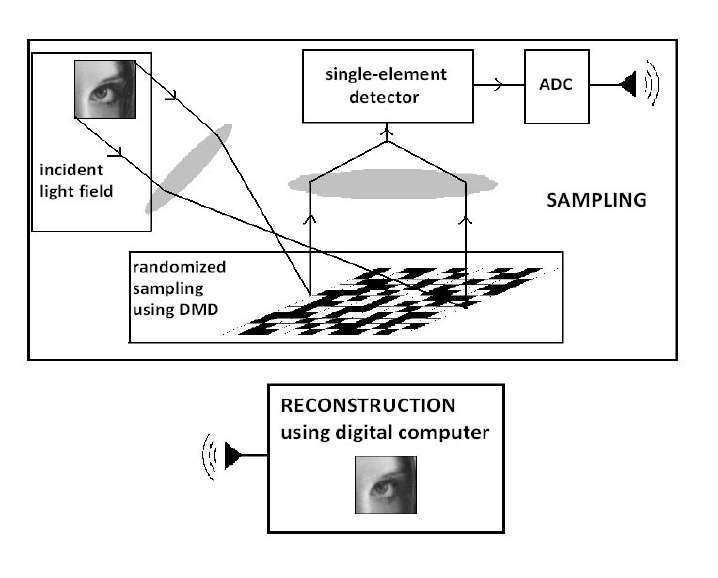
\includegraphics[height = 7 cm]{singlepixel.png}
\caption{The operation of the single pixel camera at Rice University \cite{singlepixelimaging}}
\label{singlepixelcamera}
\end{figure*}

%Compressive Sensing works best if the \(x_{i}\) are compressible (i.e. they are distributed according to a power law), and the error \(\|x - x_{s}\|\) is small.

%In Compressive Sensing measurements are taken is an incoherent basis, as opposed to the basis of the original signal. 

The question all this raises is where do we do our sensing? In other words, given that we know a basis in which our signal is sparse, \(\phi\), how do we choose \(\psi\)? It's best to choose \(\psi\) so that the signal is 'spread out' relative to the signal's expansion in \(\phi\). Such pairs are said to be incoherent. 

\begin{defn}
A pair of bases is said to be incoherent if the largest projection of two elements between the sensing (\(\psi\)) and representation (\(\phi\)) basis  is in the set \( [1 , \sqrt{n}] \), where \( n \) is the dimension of the signal. The coherence of a pair of bases is denoted by \(\mu\).
\end{defn}

This implies that sensing with incoherent systems is good (in the sine wave example above it would be better to sample randomly in the time domain as opposed to the frequency domain), and efficient mechanisms ought to acquire correlations with random waveforms (e.g. white noise).

\textbf{Theorem} \cite{Candes2006}
Fix f \(\in \mathbb{R}^n\) with a sparse coefficient basis, \(x_{i}\) in \(\psi\). Then a reconstruction from \(m\) random measurements in \(\phi\) is possible with probability \(1 - \delta\) if: 

\begin{equation}
m \geq C \mu^2(\phi, \psi) S \log\left(\frac{n}{\delta}\right)
\end{equation}
\label{minsamples}

where \( \mu(\phi, \psi)\) is the coherence of the two bases, and \(S\) is the number of non-zero entries on the support of the signal.

Then \(f*\) (the proposed reconstruction) is given by \(f^* = \psi x^*\) where \(x^*\) is the solutionn to the convex optimisation program (n.b. \(\| x\|_{l_{1}} := \sum_{i} |x_{i}| \)):

\begin{equation}
min\|\tilde{x}\|_{l_{1}} \text{ subject to } y_{k} = \left\langle \phi_{k} \text{,} \psi x^* \right\rangle \text{   } \forall k \in M \subset [1 \ldots n]
\end{equation}
\label{program0}

i.e. \textbf{CS: Sample non-adaptively in an incoherent domain and invoke linear programming after the acquisition step}

Thus the role of \(l_{1}\) minimisation is to decompress the data. There are many ways to perform this operation: some popular methods are basis pursuit \cite{Chen1998} and Greedy approaches such as Orthogonal Matching Pursuit \cite{Tropp2007}. 

It may be remarked that the \(l_0\) norm:
%
\begin{equation}
\vectornorm{l_0} = \{\# i, x_i \neq 0\}
\end{equation}
%
is a more appropriate functional to minimise. In fact under this norm, \(m \geq 2k\) measurements will suffice to uniquely determine all \(k\)-sparse signals. However, this norm is not convex and so minimising it is an NP-hard problem. As we are seeking sparse solutions the \(l_1\)-norm will suffice \cite{Donoho2006a}. This is because all vectors in a random \(k\)-dimensional subspace of an \(n\)-dimensional space are approximately Gaussian (in the sense that the components are distributed according to an approximate normal distribution). Such vectors have roughly equivalent norms, and so any solution to the \(l_1\) minimisation problem will be the same solution to the \(l_1\) minimisation problem for sufficiently sparse signals.

\subsubsection{Incoherence, isometries and all that}
To recover a sparse vector, we must make sure that the vectors are not in the null space of the sensing matrix (otherwise there would be no hope of recovery). We also require that any subset of \(S\) columns taken from the measurement matrix be nearly orthogonal w.r.t sparse vectors: i.e. all pairwise distances between S-sparse vecotrs be well preserved in the measurement space.

This can be summed up in the following inequality (Restricted Isometry Property) \cite{Emma}:

\begin{equation}
\left(1-\delta\right)\vectornorm{x}_{l_2}^2 \leq \vectornorm{Ax}_{l_2}^2 \leq \left(1+\delta\right) \vectornorm{x}_{l_2}^2
\end{equation}
\label{RIP}

We are also in a position to evaluate the meaning of the constant \(\mu\) in \ref{minsamples}. We are considering sampling within orthonormal systems (for example, Time and Frequency):
%
\begin{equation}
A*A = nI
\end{equation}
\label{orthonormal}
%
so that each row or column has \(l_2\) norm equal to \(sqrt{n}\). \(A\) is any matrix satisfying this property (examples include the Fourier matrix and the Dirac matrix). Thus \(\mu\) must be in the set \(\left[1, \sqrt{n}\right]\). \(\mu\) then, is a measure of how concentrated the rows of our measurement matrix is - i.e. how much information is spread across each vector. If \(\mu = 1\) then the rows are 'flat' -  and we need relatively fewer samples to reconstruct an S-sparse signal (i.e. each sample provides the same amount of information). However, if the rows contain all non-zero entries except for a single component, then \(\mu^2 = n\) and we will need to observe all components to determine the non-zero one (i.e. we have no guarantees of recovery from limited samples) \cite{Candes2007}. 

Noting that the measurements we take are projections from our orthonormal system (from example time) onto a sparsifying basis (i.e. frequency) we can see that:

\begin{equation}
\mu = max_{k,j} |\langle \phi_k, \psi_j \rangle |
\end{equation}
\label {mudef}
 
So we need to choose a sensing basis, where the vectors will be 'spread out', and the degree of spreading is characterised by \(\mu\).

\subsubsection{Short, Fat matrices}
As remarked upon earlier: Compressive Sensing is equivalent to solving an under-determined linear system, with the constraint that we seek the sparsest solution. The content of the previous sections amounts to constraints on the number of rows of matrix of this linear system. 

If we had an Oracle which could tell us where the non-zero components of our solution were, then we would need only as many rows of the matrix as there were non-zero components in the signal to fully specify the problem. 

%\begin{figure*}[h]
%\centering
%\includegraphics[height = 7 cm, width=\textwidth]%{compressive_sensing_example.jpg}
%\caption{A visualisation of the Compressive Sensing problem as an under-%determined system}
%\label{l1l2}
%\end{figure*}

However, such and Oracle does not exist, and so we're left with the task of constructing a matrix to recover those components. Knowing that we're looking for k-sparse solutions, we need a matrix with at least 2k columns which are linearly independent. Equivalently, all images of \(k\)-sparse vectors under the operation of the sensing matrix \(\Phi\) must be distinct. From this, any k-sparse signal can be reconstructed from \(Ax\). 

To prove this assume the opposite - then there are two vectors \(x, x' \in \mathbb{R}^n\) such that \(Ax = Ax'\). I.e. \(A(x-x') = 0\). However, \((x-x')\) is 2k-sparse and so there is a linear dependence between 2k columns of the sensing matrix A. We have a contradiction, and so 2k columns will suffice to reconstruct a k-sparse signal. 

The problem with this is that we are trying to find the support of a k-sparse signal over a vector of length N, and so we would need to check all \(N \choose k\) combinations of k-sparse signals which is prohibitively computationally expensive. Is there some way to gain the advantages of sparsity, without having to minimise a non-convex functional?

As it turns out, the answer is yes. If we take \( m \geq C \mu^2(\phi, \psi) S \log\left(n\right) \) rows minimising the \(l_{1}\) norm will find the sparsest solution. This is because the \(l_1\) norm is an octahedron (in 3-dimensions, in higher dimensions it has an analogous spiky geometry), and solutions are more likely to intersect the norm at the points. Figure \ref{l1l2} shows this.

\begin{figure*}[h]
\centering
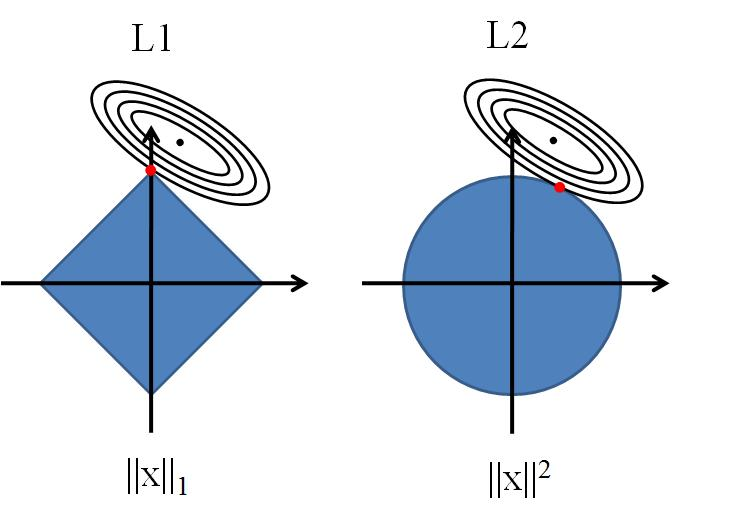
\includegraphics[height = 7 cm]{l1l2.jpg}
\caption{Solutions to the Compressive Sensing optimisation problem intersect the \(l_1\) norm the points where all components (but one) of the vector are zero (i.e. it is sparsity promoting) \cite{Tibshirani1996}}
\label{l1l2}
\end{figure*}

\subsubsection{Bayesian Compressive Sensing}
Based on the discussion above we can represent the compressive sensing measurements as: 

\begin{equation}
\textbf{g} = \Phi	\textbf{w}
\end{equation}

where \(\Phi\) is a \(K \times	N\) matrix which is the product of the measurement and sparse bases described earlier.

Note that the measurements may be noisy, with the measurement noise represented by a zero mean Gaussian distribution and unknown variance \( \sigma^2 \):

\begin{equation}
\textbf{g} = \Phi \textbf{w} + \textbf{n}
\end{equation}
\label{CSequation}

Where \textbf{n} is the vector representing the vector of noise, and has the same support as the measurements. 

Previous sections have shown how the weights \(w\) may be found through optimisation methods such as basis pursuit or greedy algorithms. Here, an alternative Bayesian model is described.

From \ref{CSequation} we have a Gaussian likelihood model: 

\begin{equation}
p \left( \textbf{g} \mid \textbf{w}\text{,} \sigma^2 \right) = (2 \pi \sigma^2)^{-K/2} \exp{\left(- \frac{1}{2 \sigma^2} \|\textbf{g} - \Phi	\textbf{w}\|_{2}^{2} \right)} 
\end{equation}

The above has converted the CS problem of inverting sparse weight \textbf{w} into a linear regression problem with a constraint (prior) that \textbf{w} is sparse. 

To seek the full posterior distribution over \textbf{w} and \( \sigma^2 \), we can chose a sparsity promoting prior. A popular sparseness prior is the Laplace density functions:

\begin{equation}
p\left(w\mid\lambda\right) = \left(\frac{\lambda}{2}\right)^N exp{-\lambda \sum_{i=1}^{N} |w_i|}
\end{equation}

Note that the solution the convex optimisation problem \ref{program0} corresponds to a maximum \textit{a posteriori} estimate for \(w\) using this prior. I.e this prior is equivalent to using the \(l_1\) norm as an optimisation function (see figure \ref{laplacenormal} \cite{Tibshirani1996}).

\begin{figure*}[h]
\centering
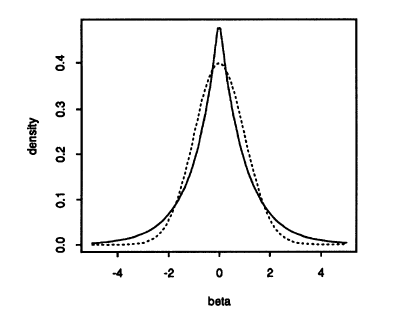
\includegraphics[height = 7 cm]{LaplaceandNormalDensity.png}
\caption{The Laplace (\(l_1\)-norm, bold line) and Normal (\(l_2\)-norm, dotted line) densities. Note that the Laplace density is sparsity promoting as it penalises solutions away from zero more than the Gaussian density. \cite{Tibshirani1996}}
\label{laplacenormal}
\end{figure*}

The full posterior distribution on \(w\) and \(\sigma^2\) may be realised, by using a hierarchical prior instead. To do this, define a zero-mean Gaussian prior on each element of \(w\):
%
\begin{equation}
p\left(w\mid a\right) = \prod_{i=1}^{N}\mathbb{N}\left(w_i\mid 0, \alpha_{i}^-1\right)
\end{equation}
%
where \(\alpha\) is the precision of the distribution. A gamma prior is then imposed on \(\alpha\):

\begin{equation}
p\left(\alpha \mid a, b \right) = \prod_{i=1}^{N} \Gamma\left( \alpha_i \mid a, b \right)
\end{equation}

The overall prior is found by marginalising over the hyperparameters:

\begin{equation}
p\left( w \mid a, b \right) = \prod_{i=1}^{N} \int_{0}^{\infty} \mathbb{N}\left(w_i\mid 0, \alpha_{i}^-1\right) \Gamma\left( \alpha_i \mid a, b \right)
\end{equation}

This integral can be done analytically and is a Student-t distribution. Choosing the parameters \(a,b\) appropriately we can make the Student-t distribution peak strongly around \(w_i = 0\) i.e. sparsifying. This process can be repeated for the noise variance \(\sigma^2\). The hierarchical model for this process is shown in \ref{bayesiancs}. This model, and other CS models which not necessarily have closed form solutions, can be solved via belief-propagation \cite{Baron2010}

\begin{figure*}[h]
\centering
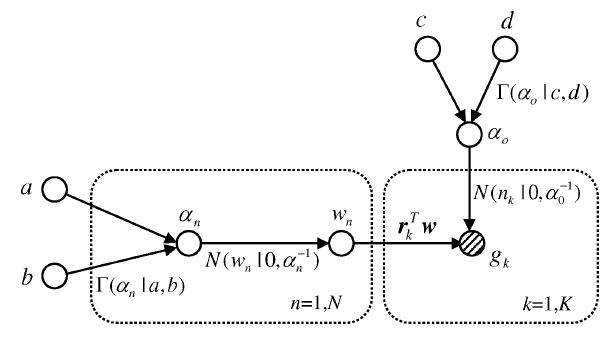
\includegraphics[height = 7 cm]{bayesiancs.png}
\caption{The hierarchical model for the Bayesian CS formulation \cite{Ji2008}}
\label{bayesiancs}
\end{figure*}

\subsubsection*{OMP}

\begin{algorithm}[H]

 \SetKwData{Left}{left}\SetKwData{This}{this}\SetKwData{Up}{up}
 \SetKwFunction{Match}{match}\SetKwFunction{Update}{update}
 \SetKwInOut{Input}{input}\SetKwInOut{Output}{output}

 \Input{Observation vector \(\textbf{y}\), sensing matrix \(\textbf{A}\), stopping criterion \(s\)}
 initialization \\
 \(k \leftarrow 0\) \\
 \(\Lambda_0 = \emptyset\) \\
 \(\textbf{r}_k \leftarrow \textbf{y}\) \;
 \While{\(k \neq s\) or \(\textbf{r}_k \neq 0 \)}{
   \(k \leftarrow k+1\)\;
   \Match{\(h_k = A^T \textbf{r}^{k-1}\)}\;
   \(\Lambda_k = \Lambda_{k-1} \cup \argmin_j{h_k\left(j\right)} \)\;
  \Update:\;
  \(\hat{\textbf{x}} \leftarrow \textbf{A}_{\Lambda_k}^\dagger \textbf{y}\)\;
  \(\textbf{r}_k \leftarrow \textbf{y} - \textbf{A}_{\Lambda_k}^\dagger \textbf{y} \)
 }
 \Output{\(\hat{\textbf{x}} = \argmin_{x:\supp\left(x\right) \subseteq  \Lambda_k}\|y-Ax\|_2\)}
 \caption{Orthogonal Matching Pursuit}
\end{algorithm}

OMP iteratively detects the support set of the signal - proceeding by extending the estimate by a single index per iteration. The algorithm uses a matched filter to find the column which is maximally correlated with the current estimate, and solves a least-squares problem to update the residual vector.

Remarks:
\begin{itemize}
\item The residual vector at step \(k\), \(\textbf{r}_k\), can be viewed as the orthoganalisation of the observation vector against the previously chosen columns of \(\textbf{A}\).
\end{itemize}

\subsection{Group Testing}
Group Testing originated in the second world war because of the need to test all incoming conscriptees for syphilis. It would have been inefficient and expensive to test each soldier individually, as the rate for syphilis was only 10 per 100,000. Dorfman \cite{Dorfman1943}, considered the idea of pooling blood samples and testing the pooled samples for syphilis and only further testing the pools which come up positive.

A typical problem that can be solved by Group Testing is finding a counterfeit coin in a group of otherwise identical coins by weighing groups of coins on a pan balance. For example, given 80 coins known to contain a single counterfeit, which is lighter than the others, what is the minimum number of weighings needed to determine the counterfeit with certainty? You may get lucky and pick the counterfeit in the for the first go: but there's only a \(\frac{1}{80}\) chance of that happening. There's also no need to check all \(80 \choose 1\) combinations of pairs of coins. However, putting more than one coin on a pan reveals the same information  - it's better to weigh groups of coins against each other.

Choose the groups so that each weighing can distinguish between the hypothesis that the pans will balance, or than there will be a heavier pan i.e. split the initial group into 3 (27, 27, 26). Continue this process recursively, splitting the remaining group into 3 each time, until you have found the counterfeit. If the two groups of 27 balance initially, take a coin from one of those groups and add it to the group of 26 to make a power of 3. This won't add any new information (you know this coin is not counterfeit) and so won't affect the inference.

The Group Testing problem can be formalised as follows: a set of items is given, along with an upper bound on the number of defectives. The set is described as a vector, where if an item is 0 it is not defective and 1 if it is defective. Before the tests are run, the position of the 1's is unknown. 

To find the defective items, a query is run against a subset of \([n]\), where the answer is defined as follows:

\begin{equation}
A\left(S\right) = 1 \sum_{i} x_i \geq 1
\end{equation}

Note that the addition is the binary-or in the above summation. The goal of Group Testing is to minimise the number of tests required to reconstruct the defective set.

\subsubsection*{Algorithms}
An initial algorithm to consider is a simple binary search of the set to be tested. That is, given a set of size \(N = 2^r\) i.e a powre of 2, we can recover a single defective in
\(\lceil{\log_2{N}}\rceil\) tests.

To do this, create a new set of size \(S = 2^{\lceil{\log_2{n}}\rceil}\) which is guaranteed to contain a defective. Label the items with integers, and test the items in the sets \({1,2,\ldots ,S/2}\) and \({S/2 + 1,\ldots ,S/2}\) separately. Then repeat the procedure on any groups which have a positive test. 

To see why this testing procedure takes at most \(\lceil{\log_2{n}}\rceil\) tests, note that the procedure defines a binary tree over subsets of the N items, and so the depth of this tree is \(\lceil{\log_2{N}}\rceil\).

For input sets with more than a single defective (say \(K\) defectives) the binary search algorithm can be repeated, and each time a defective is found it is removed from the set. The binary search is then repeated, but on a set of size \(N-1\). Using this procedure we are guaranteed to find all the defectives in 

\begin{equation}
K \lceil \log_2{N} \rceil \leq K\log_2{N} + K
\end{equation}

tests. However, this is a very inefficient algorithm: early sets are large and so are likely to contain a defective.

The above algorithms return, with certainty, after at most \(K\lceil \log_2{N\choose K}\rceil\) tests, the defective set. Much work has gone into combinatorial search algorithms, often more complex than those described above. 

This has been motivated by the analogy that the Group Testing problem can be considered a decoding problem where an experimenter receives a binary vector: 

\begin{equation}
y = \textbf{A}x
\end{equation}

\(y \in \{0,1\}^K, x \in \{0,1\}^N\), and wishes to decode the vector \(x\) to recover the defective set, subject to the constraints of the testing matrix \(\textbf{A}\). The matrix has to satisfy the property that the Boolean sum of any \(t\) columns was unique, and did not contain any other column in the matrix. These properties are known as seperability and disjunctness. 

\begin{figure*}[h]
\centering
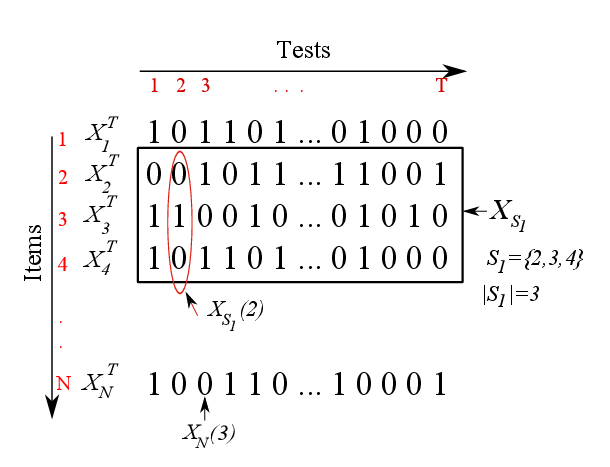
\includegraphics[height = 7 cm]{GTFat.png}
\caption{The Group Testing model: multiplication with a short, fat matrix \cite{Atia2008}}
\label{bayesiancs}
\end{figure*}

See (REF HWANGDU) for more a detailed introduction and analysis of the requisite algorithms.

\subsubsection*{Hwang's Algorithm}
In modern Coding Theory, there has been a move away from exlicit combinatorial algorithms which return the codeword with certainty, towards probabalisitic algorithms which return the correct codeword with an associated probability. The advantage of this has been the development of algorithms which can decode codes close to the Shannon capacity of the channel.

Similarly in Group Testing, the state of the art considers probabilistic algorithms instead of explicit combinatorial designs. 

The problems with the binary search algorithm (that initial groups are very large and are highly likely to contain a defective) above can be overcome by instead considering groups whose size is chosen so that the probability that the group will have a positive test is close to half. Equivalently, given a set of size \(N=2^r\) which are known to contain K defectives, in expectation a group of size \(\frac{K}{N}\) should contain a defective. 

Thus we can use fewer tests than predicted by simple repeated binary search, by testing 'pilot' groups of size roughly \(\frac{K}{N}\). Hwang \cite{Hwang1972} gives such an algorithm, and provides an upper bound on the number of tests required to recover the defective set.

The steps for the algorithm are:

\begin{enumerate}
\item If \(n \leq 2d-2\) then test every item individually. Otherwise set \(l = n - d + 1\) and define \(\alpha:=\log{\lceil \frac{l}{d}\rceil}\).
\item Test a group of size \(2^\alpha\). If the outcome is negative, the groups is good. Set \(n := n - 2^\alpha \) and go to 1. If the outcome is positive, then use binary splitting on the group to identify a defective and \(x\) good items. Set \(n := n - 1 -x \) and \(d:= d-1\) and go to 1.
\end{enumerate}

The upper bound on the number of tests is given by the following argument: as there are \(n \choose k\) possible sets of defectives, and in \(t\) tests at most \(2^t\) cases can be differentiated, \(\lceil \log_2{n \choose k} \rceil\) tests are needed. 

\subsubsection*{Bounds}
It has been previously believed that the success probability to recover the defective set given \(T\) tests was:

\begin{equation}
P\left(Success\right) \leq \frac{T}{\log_2{N \choose K}}
\end{equation}

However, a tighter upper bound has recently been found \cite{Aldridge2013} at:
%
\begin{equation}
P\left(Success\right) \leq \frac{2^T}{ {N \choose K} }
\end{equation}
%
i.e. the probability of success increases exponentially with the number tests, opposed to linearly. 

In the Group Testing literature there exists an 'adaptivity gap' - it seems that adaptive algorithms \textit{do} give a performance improvement over non-adaptive algorithms, in terms of the number of tests required to recover the defective set. This is discussed here, using Hwang's algorithm as a test bed.

Hwang's algorithm is guaranteed to succeed in:

\begin{equation}
T = \log_2{N\choose K} + K
\end{equation}

tests. The Combinatorial Orthogonal Matching Pursuit algorithm, considered in \cite{Chan2011}, is guaranteed to recover the defective set with probability \(N^{-\delta} \) in
%
\begin{equation}
T = \left(\left(1+\delta\right)e\right)K\ln{N}
\end{equation}
%
tests. For all \(N\) and \(K)\) we have:
%
\begin{equation}
K\log_2{\frac{N}{K}} \leq \log_2{N \choose K} \leq K \log_2{\frac{Ne}{K}}
\end{equation}
%
which follows from well-know bounds on binomial coefficients. This allows a contrast between the asymptotic bounds of previous algorithms to be considered in this section. We see that, the regime where \(K = N^{1-\beta}\), Hwang's algorithm succeeds with:
%
\begin{equation}
T = \beta K \log_2{N} + K\left(\log_2{e} + 1\right)
\end{equation}
\label{hwangbound}
%
tests, whilst the COMP algorithm succeeds with:
%
\begin{equation}
1.88\left(1+\delta\right)K\log_2{N}
\end{equation}
\label{compbound}
%
tests. It's worthwhile to contrast these results, to gain some insight into the problem. \ref{hwangbound} suggests that for very sparse problems (\(\beta\) tending towards 1) that Hwang's adaptive algorithm will outperform a simmilar non-adaptive algorithm. Even though the two procedures have the same complexity, they have different constants (1 v,s 1.88 in the sparse case). Thus, there are asymptotic gains (in terms of the number of tests required to recover the defective set) which are offered by adaptive algorithms, and not by non-adaptive algorithms.

These ideas can be summarised in the idea of a \textit{capacity} for Group Testing \cite{Baldassini2013}. That is, there is a constant \(C\) such that a sequence of Group Testing algorithms with \( K = \omega\left(N\right)\) will succeed with probability tending to 1. This allows different noise, and dilution models to be considered so that a more complete characterisation of the structural properties of Group Testing is revealed.
 
\subsubsection{Comparison to Compressive Sensing}
The goal of Coding Theory is given a vector \(x \in \mathbb{F}^m\), where \(\mathbb{F}\) is some finite-field, is to construct a 'code-book' \(C\) which produces a vector \(y \in \mathbb{F}^n\), \(n > m\), so that the original vector may be transmitted over a noisy-channel with vanishing error probability. This problem is structurally similar to the Compressive Sensing and Group Testing problems, but in reverse. In CS and GT we're given 'short' vector, and we wish to infer the 'longer' one satisfying the constraint that we seek the sparsest vector, under some conditions on the matrix \(\Phi\). This suggests that there may be some Information-theoretic framework uniting all three disciplines. 

In \cite{Emma} Tao and Candes consider the CS problem as one of error correction of a linear code: however in this case the codewords are drawn from \(\mathbb{R}^m\) as opposed to a finite alphabet more common in Coding Theory. This is done by considering \(\Phi\) as the parity check matrix of a linear code and the signal x as the error pattern. Linear programming can then be viewed as a method for decoding. 

Group testing is a combinatorial variant of Compressive Sensing, where the sensing matrix is a binary matrix. The matrix represents combinations (or pools) of items, such that a 1 in the \(i^{th}\) row and \(j^{th}\) column means that  the \(i^{th}\) item is tested in the \(j^{th}\) pool. The goal of Group testing can then be seen as designing testing pools so to accurately reconstruct the sparse set of interesting items. 

In Group Testing, instead of the sensing matrix being to subject to coherence constraints such as those above, the sensing matrices have the property that the support of any column is not contained in the union of the supports of any t other columns. Thus a t-disjunct matrix defines a group testing scheme which an identify any defective set up to size t.

The analogue between Group Testing and Coding is even closer, as GT explicitly considers signals and matrices from Binary alphabets. That is, Group Testing is a closer cousin of Coding Theory than Compressive Sensing, in a sense the inverse problem as in both Coding and Group Testing we are working over a finite field. This is encouraging, as it could allow the reconstruction of the defective set via methods developed in Coding Theory. There has been some work done on this, \cite{Sejdinovic2010} considers the noisy Group Testing problem and the reconstruction of the defective set via belief propagation whilst \cite{Wadayama2013} gives explicit theorems on conditions for the recovery of the defective set for the case of the binary symmetric channel. \cite{Baldassini2013} takes this further and finds the capacity of Group Testing for a number of cases. 

\subsection{The Probabilistic group testing problem}
Group testing is a sparse inference problem, first introduced by Dorfman \cite{dorfman} in the context of testing for rare diseases.
Given  a large population of items \(\setP\),
indexed by \( \{1, \ldots N\}\), where
some small fraction of the items are interesting in some way, how can we find the interesting items efficiently? 

We perform a sequence of $T$ pooled tests defined by test sets $\setX_1, \ldots, \setX_T$, where each $\setX_i \subseteq \setP$. 
We represent the interesting (`defective') items by 
a random vector $\vc{U} = ( U_1, \ldots, U_N)$, where $U_i$ is the indicator of the event that item $i$ is defective. 
For each test $i$, we jointly 
test all the items in $\setX_i$, and the outcome $y_i$ is `positive' ($y_i = 1$) if and only if any item in $\setX_i$ is defective. In other words, 
$y_i = \II \left( \sum_{j \in \setX_i} U_j \right)$, since for simplicity we are  considering the noiseless case. Further, in this paper, we restrict our attention to
 the adaptive case, where we choose test set
$\setX_i$ based on a knowledge of sets $\setX_1, \ldots, \setX_{i-1}$ and outcomes $y_1, \ldots, y_{i-1}$. The group testing problem requires us to infer $\vc{U}$ with high
probability given a low number of tests $T$.

Since Dorfman's paper \cite{dorfman}, there has been considerable work on the question of how to design the sets $\setX_i$ in order to minimise the number of tests $T$
required. In this context, we briefly mention so-called combinatorial designs (see \cite{du, malyutov} for a summary, with \cite{malyutov} giving invaluable
references to an extensive body of Russian work in the 1970s and 1980s). Such designs typically aim to ensure that 
set-theoretic properties known as disjunctness
and separability occur. In contrast, for simplicity of analysis, as well as  performance of optimal order, it is possible to consider random designs. Here sets $\setX_i$ are chosen
at random, either using constructions such as independent Bernoulli designs \cite{atia, johnsonc8, johnson33} or more sophisticated  random designs based on LDPC codes \cite{wadayama}. 

Much previous work has focussed on the Combinatorial group testing problem, where there are a fixed number of defectives $K$, and the defectivity vector $\vc{U}$ is chosen uniformly among all
binary vectors of weight $K$. In contrast, in this paper we study a Probabilistic group testing problem as formulated
for example in the work of Li et al. \cite{li5}, in that we suppose 
 each item is defective  independently with probability \(p_i\), or equivalently take $U_i$ to be independent Bernoulli($p_i$).

This Probabilistic framework, including non-uniform priors, is natural for many applications of group testing.
For example, see \cite{atia2}, the cognitive radio problem can be formulated in terms of  a population
 of communication bands in frequency spectra with some (unknown) occupied bands you must not utilise. Here, the values of $p_i$ may be chosen
 based on some database of past spectrum measurements or other prior information. Similarly, as in Dorfman's original work  \cite{dorfman} or more recent 
research \cite{shental} involving screening for genetic conditions, values of
$p_i$ might summarise prior information based on a risk profile or  family history.
%
\subsection{Group testing capacity}
%
It is possible to characterize performance tradeoffs in group testing 
 from an information-theoretic point of view -- see for example \cite{atia, johnsonc10, johnson33, tan}. These papers have focussed on group testing as a channel coding problem, 
with \cite{atia, tan}
explicitly calculating the mutual information.
The paper \cite{johnsonc10} defined the capacity of a Combinatorial group testing procedure, which characterizes the number of bits of information
about the defective set which we can learn per test. We give a more general definition here,
which covers both the Combinatorial and Probabilistic cases.
%
\begin{definition} \label{def:capacity} Consider a sequence of group testing problems where the $i$th problem
has defectivity vector  $\vc{U}^{(i)}$, and consider algorithms which are given $T(i)$ tests.
We refer to a constant $C$ as the (weak) group testing capacity if for any $\epsilon > 0$:
  \begin{enumerate}
    \item any sequence of algorithms with
      \begin{equation} \label{eq:lower}
        \liminf_{i \tends} \frac{ H(\vc{U}^{(i)}) }{T(i)} \geq C+ \epsilon,
      \end{equation}
      has success probability $\pr(\suc)$ bounded away from 1,
    \item and there exists a sequence of algorithms with
      \begin{equation} \label{eq:upper}
        \liminf_{i \tends} \frac{H(\vc{U}^{(i)}) }{T(i)}  \geq C - \epsilon
      \end{equation}
      with success probability $\pr(\suc) \rightarrow 1$.
  \end{enumerate}
\end{definition}
%
\begin{remark}
In the Combinatorial case of $K$ defective items with all defective sets equally
likely, $ H(\vc{U}) = \log_2 \binom{N}{K}$, which is the term found in the denominator in \cite[Eq. (1) and (2)]{johnsonc10}. In the Probabilistic case (as in \cite{li5}) 
 we know $H(\vc{U}) = -\sum_{i=1}^N h(p_i)$ where $h(t) = -t \log_2 t - (1-t) \log_2(1-t)$ is the binary entropy function. 
\end{remark}
%
\begin{remark} If for $ \liminf_{i \tends} \frac{ H(\vc{U}^{(i)}) }{T(i)} \geq C+ \epsilon$, the success probability 
$\pr(\suc) \rightarrow 0$ we say that $C$ is the strong group testing capacity, following standard terminology in information
theory. Such a result is referred to as a strong converse.
\end{remark}

\subsection{Main results}

The principal contribution of \cite[Theorem 1.2]{johnsonc10} was the following result:
%
\begin{theorem}[\cite{johnsonc10}] \label{thm:mainold}
The strong capacity of the adaptive noiseless Combinatorial group testing problem
  is  $C = 1$,
  in any regime such that $K/N \rightarrow 0$.
\end{theorem}
%
This argument came in two parts. First, in \cite[Theorem 3.1]{johnsonc10} the authors  proved a new
upper bound on success probability 
\begin{equation} \label{eq:bja} \pr(\suc) \leq \frac{2^T}{\binom{N}{K}}, \end{equation} which implied a strong converse ($C \leq 1$). This was complemented 
by 
showing that, in the Combinatorial case, an algorithm based on 
Hwang's Generalized Binary Splitting Algorithm (HGBSA) \cite{hwang}, \cite{du} is essentially optimal in the required sense,
showing that $C=1$ is achievable.


It may be useful to characterize the Probabilistic group testing problem in 
terms of the effective sparsity $\mu^{(N)}: = \sum_{i=1}^N p_i$. In particular, if the $p_i$ are (close to) identical, we would expect performance similar to that in the Combinatorial
case with $K = \mu^{(N)}$ defectives. As in \cite{johnsonc10}, we  focus on asymptotically sparse cases, where $\mu^{(N)}/N \rightarrow 0$ (in contrast, Wadayama
\cite{wadayama} considered a model where $p_i$ are identical and fixed).
The main result of the present paper is Theorem \ref{thm:main}, stated and proved in Section \ref{sec:main} below, which implies the 
following  Probabilistic group testing version of Theorem \ref{thm:mainold}.
 %
\begin{corollary} \label{cor:main}
 In the case where $p_i \equiv p$, the weak capacity of the adaptive noiseless Probabilistic group testing problem
  is  $C = 1$, in any regime such that $\mu^{(N)}/N \rightarrow 0$ and $\mu^{(N)} \rightarrow \infty$.
  \end{corollary}



Again we prove our main result Theorem \ref{thm:main} using complementary bounds on both sides. First in Section \ref{sec:ub} we recall
 a universal upper bound on success probability, Theorem \ref{thm:upper}, taken from
\cite{li5}, which implies a weak converse.   In \cite{li5}, Li et al. introduce
the Laminar Algorithm for Probabilistic group testing.  
In Section \ref{sec:algo} we propose a refined version of this Laminar Algorithm, based on Hwang's HGBSA \cite{hwang}, which is
analysed in Section \ref{sec:main}, and shown to imply performance close to optimal in the sense of capacity.

\section{Algorithms and existing results}

\subsection{Upper bounds on success probability} \label{sec:ub}

Firstly \cite[Theorem 1]{li5} can be restated to give the following
upper bound on success probability:
%
\begin{theorem} \label{thm:upper}
Any Probabilistic group testing algorithm using $T$ tests with noiseless measurements has success probability satisfying
$$ \pr(\suc) \leq \frac{T}{H( \vc{U})}.$$
\end{theorem}

Rephrased in terms of Definition \ref{def:capacity}, this tells us that the weak capacity of noiseless Probabilistic 
group testing is $\leq 1$. The logic is as follows; if the capacity were
$1 + 2 \epsilon$ for some $\epsilon > 0$, then there would exist a sequence of algorithms with $H(\vc{U}^{(i)})/T(i) \geq 1 + \epsilon$ with success probability tending to 1.
However, by Theorem \ref{thm:upper}, any such algorithms have $\pr(\suc) \leq 1/(1+\epsilon)$, meaning that we have 
established that a weak converse holds.

\begin{remark}
It remains an open and interesting problem to prove an equivalent of \eqref{eq:bja} as in \cite[Theorem 3.1]{johnsonc10}. That is we hope to find an upper bound
on success probability in a form  which implies a strong converse, and hence that the strong capacity of Probabilistic group
testing is equal to 1.
\end{remark}

\subsection{Binary search algorithms}

The main contribution of this work is  to describe and analyse algorithms that will find the defective items.
In brief, we can think of Hwang's HGBSA algorithm as dividing the population $\setP$ into search sets $\setS$. First, all the items in a search set $\setS$ are tested together,
using a test set $\setX_1 = \setS$. If the result is negative
($y_1 = 0$), we can be certain that $\setS$ contains no defectives. However, if the result is positive ($y_1 = 1$),  $\setS$ must contain at least one defective.

If $y_i = 1$, we can be guaranteed to find at least
one defective, using the following binary search strategy.  
We  split the   set $\setS$ in two, and test the `left-hand' set, say $\setX_{2}$. If $y_{2} = 1$, then we know that $\setX_{2}$ contains at least one defective.
If $y_{2} = 0$, then $\setX_{2}$ contains no defective, so we can deduce that $\setS \setminus \setX_2$ contains at least one defective. By repeated use of this strategy, we are 
guaranteed to find a succession of nested sets which contain at least one defective, until $\setX_i$ is of size 1, and we have isolated a single defective item.

However this strategy may not find every defective item in $\setS$. To be specific, it is possible that at some stage
both the left-hand and right-hand sets contain a defective. The Laminar Algorithm of \cite{li5} essentially deals with this by testing 
both sets. However, we believe that this is inefficient, since typically both sets will not contain a defective. Nonetheless, the Laminar Algorithm satisfies
 the following  performance guarantees  proved in \cite[Theorem 2]{li5}: 
%
\begin{theorem} \label{thm:lower}
The expected number of tests required by the Laminar Algorithm \cite{li5}  is $\leq 2 H(\vc{U}) + 2 \mu$. Under a technical condition (referred to as non-skewedness), the
success probability can be bounded by $\pr(\suc) \geq 1- \epsilon$ using $T = (1+ \delta) (2^{\Gamma + \log_2 3} + 2) H(\vc{U})$ tests, where $\Gamma$ is defined implicitly
in terms of $\epsilon$, and $\delta \geq 2 e - 1$.
\end{theorem}

Ignoring the $\Gamma$ term, and assuming the non-skewedness condition holds,
 this implies that (using the methods of \cite{li5}) $T =  2 e (3 + 2) H(\vc{U}) = 10 e H(\vc{U})$ tests are required to guarantee convergence to $1$
of the success probability. In our language, this implies a lower bound of $C \geq 1/(10 e) = 0.0368$. Even ignoring the analysis of error probability, the fact that the expected number
of tests is $\leq 2 H(\vc{U}) + 2 \mu$ suggests that we cannot hope to achieve $C > 1/2$ using the Laminar Algorithm.
%
\subsection{Summary of our contribution} \label{sec:algo}

\begin{algorithm}
 \SetLine 
 %\SetAlgoLined % For previous releases [?]
 \KwData{A Set \(S\) of \(\lvert S \rvert = n\) items, \(\mu\) of which are actually defective in expectation, a probability vector \( \vec{p}^{\left(n\right)} \) describing each item's independent probability of being defective, and a cutoff \(\theta\)}
 \KwResult{The set of defective items}
 Discard items with \(p_i \leq \theta\)
 \\
 Sort the remaining items into \(B\) bins, collecting items together with \(p_i \in \left[1/2C^r,1/2C^{r-1}\right)\) in bin \(r\).
 \\
 Sort the items in each bin into sets s.t. the (normalised) probability of each set is less than \(1/2\).
 \\
 Test each set in turn
 \\
   	\If{The test is positive}{Arrange the items in the set on a Shannon-Fano/Huffman Tree and search the set for all the defectives it contains}

 \caption{Algorithm for the non-iid group testing problem}
\end{algorithm}

The main contribution of our paper is a refined version of the Laminar Algorithm, summarised above, and an analysis resulting in tighter error bounds as formulated in Proposition \ref{prop:overall} (in terms of expected number of tests) and Theorem \ref{thm:main} (in terms
of error probabilities).
The  key ideas are:
\begin{enumerate}
\item To partition the population $\setP$ into search  sets  $\setS$ containing items which have similar probabilities,
expressed through the Bounded Ratio Condition \ref{cond:ratio}. This is discussed in Section \ref{sec:boundedratio}, and optimised in the proof
of Proposition \ref{prop:overall}.
\item The way in which we deal with sets $\setS$ which contain more than one defective, as discussed in Remark \ref{rem:algo} below. Essentially we do not backtrack after each test by
testing both left- and right-hand sets, but only backtrack after each defective is found.
\item To discard items which have probability below a certain
threshold, since with high probability none of them will be defective. This is an idea introduced in \cite{li5} and discussed
in Section \ref{sec:discard}, with a new bound given in Lemma \ref{lem:thresh}.
\item  Careful analysis in Section \ref{sec:expectation} of the properties of search sets $\setS$ gives Proposition \ref{prop:overall}, which shows that the expected number of tests required can
be expressed as $H(\vc{U})$ plus an error term. In Section \ref{sec:main},
we give an analysis of the error probability using Bernstein's inequality, Theorem \ref{thm:bernstein}, allowing us to
prove Theorem \ref{thm:main}.
\end{enumerate}
%


\subsection{Wider context: sparse inference problems}

Recent work \cite{aksoylar,tan} has shown that many arguments and bounds hold in a common framework of sparse inference
which includes group testing and compressive sensing.

Digital communications, audio, images, and text are examples of data sources we can compress. We can do this, because these data sources are sparse: they have fewer degrees of freedom than the space they are defined upon. 
For example, images have a well known expansion in either the Fourier or Wavelet bases. The text of an English document will only be comprised of words from the English dictionary, and not all the possible strings from the space of strings made up from the characters \(\{a, \ldots, z \}\). 

Often, once a signal has been acquired it will be compressed. However, the compressive sensing paradigm introduced by
\cite{candes,donoho2} shows that this isn't necessary. In those papers it was shown that a 'compressed' representation of a signal could be obtained from random linear projections of the signal and some other basis (for example White Gaussian Noise). The question remains, given this representation how do we recover the original signal? For real signals, a simple linear programme suffices.
Much of the work in this area has been couched in terms of the sparsity of the signal and the various bases the signal can be represented in (see for example \cite{candes,donoho2}). 


\section{Analysis and new bounds}

\subsection{Searching a set of bounded ratio} \label{sec:boundedratio}

Recall that we have a population $\setP$ of items to test, each with associated probability of defectiveness $p_i$.
The strategy of the proof is to partition $\setP$ 
 into search sets $\setS_1, \ldots, \setS_G$, each of which contains items which have
comparable values of $p_i$.

\begin{condition}[Bounded Ratio Condition] \label{cond:ratio}
Given $C \geq 1$, say that a set $\setS$ satisfies the Bounded Ratio Condition with constant $C$ if
\begin{equation} \label{eq:ratio} \max_{i,j \in \setS} \frac{p_j}{p_i} \leq C.\end{equation} \end{condition}
%
(For example clearly if $p_i \equiv p$, any set $\setS$ satisfies the condition for any $C \geq 1$).
%
\begin{lemma} \label{lem:sfstep}
Consider a set $\setS$ satisfying the Bounded Ratio Condition  with constant $C$
and write $P_{\setS} = \sum_{j \in \setS} p_j$.
In a  Shannon--Fano tree for the probability distribution $\ol{p}_i := p_i/P_{\setS}$, each item has length $\ell_i^{(\setS)}$
bounded by
\begin{equation} \label{eq:depth} \ell_i^{(\setS)} \leq \ell_{\max}^{(\setS)} := \frac{h(\setS)}{P_{\setS}} + \log_2  C + \log_2  P_{\setS} + 1,\end{equation}
where we write $h( \setS) :=  -\sum_{j \in \setS} p_j \log_2  p_j$.
\end{lemma}
\begin{IEEEproof}
Under the Bounded Ratio Condition, for any $i$ and $j$, we know that by taking logs of \eqref{eq:ratio}
$$ -\log_2 p_i \leq - \log_2 p_j + \log_2 C.$$
Multiplying by $p_j$ and summing over all $j \in \setS$, we obtain that
\begin{equation} \label{eq:setbd} -P_{\setS} \log_2 p_i \leq h(\setS) + P_{\setS} \log_2 C.\end{equation}
Now, the Shannon--Fano length of the $i$th item is
\begin{eqnarray}
 \ell_i^{(\setS)}  = \lceil -\log_2 \ol{p}_i \rceil 
& \leq &  -\log_2 p_i + \log_2 P_{\setS} + 1 \label{eq:lengthbd} \\
& \leq  & \left(\frac{h(\setS)}{P_{\setS}} + \log_2 C \right) + \log_2 P_{\setS} + 1. \nonumber
\end{eqnarray}
and the result follows by \eqref{eq:setbd}.
\end{IEEEproof}

Next we describe our search strategy:

\begin{remark} \label{rem:algo}
Our version of the algorithm will find every defective in a set $\setS$. We start as before by testing every item in $\setS$ together. If this test is negative, we are done.
Otherwise, if it is positive, we can perform binary search as above to find one defective item, say $d_1$. Now, test every item in $\setS \setminus \{ d_1 \}$ together.
If this test is negative, we are done, otherwise we repeat the search step on this smaller set, to find another defective item
$d_2$, then we test $\setS \setminus \{ d_1, d_2 \}$ and so on.

We think of the algorithm as repeatedly searching a binary tree. Clearly, if the tree has depth bounded by $\ell$, then the search will take $ \leq \ell$ tests to find one defective. In total, 
if the set contains $U$ defectives, we need to repeat $U$ rounds of searching, plus the final test to guarantee that the set contains no more defectives, so will use $\leq \ell U + 1$ tests.
\end{remark}

\begin{lemma} \label{lem:expset}
 Consider a search set $\setS$ satisfying the Bounded Ratio Condition  and write $P_{\setS} = \sum_{j \in \setS} p_j$.
If (independently) item $i$ is defective with probability $p_i$, 
we can recover  all defective items in the set using $T_\setS$ tests, where $\ep T_\setS \leq T_{\bd}(\setS)$ for
\begin{equation} \label{eq:tbds}
 T_{\bd}(\setS) :=  h(\setS) +  P_{\setS} \log_2 C +  P_{\setS} \log_2 P_{\setS} + P_\setS + 1. \end{equation}
\end{lemma}
\begin{IEEEproof}
Using the algorithm of Remark \ref{rem:algo}, laid out on the Shannon-Fano tree constructed in Lemma \ref{lem:sfstep}, we are guaranteed  to find every defective.
The number of tests to find one defective thus corresponds to the depth of the tree, which is bounded by  $\ell_{\max}^{(\setS)}$ given in \eqref{eq:depth}.

Recall that we write $U_i$ for the indicator of the event that the $i$th item is defective, $U_{\setS} = \sum_{i \in \setS} U_i$ and 
$l_i^{(\setS)}$ for the length of the word in the Shannon Fano tree. As discussed in Remark \ref{rem:algo}
this search procedure will take 
\begin{eqnarray}
T_\setS & = &  1 + \sum_{i \in \setS} U_i \ell_i^{(\setS)} \nonumber \\
& = &  \sum_{i \in \setS} p_i \ell_i^{(\setS)} + 1 + \sum_{i \in S} \ell_i^{(\setS)} (U_i - p_i)  \nonumber \\
& \leq & \sum_{i \in \setS} p_i \ell_{\max}^{(\setS)} +  1 + \sum_{i \in \setS} V_i^{(\setS)}  \nonumber \\
& =  &  P_{\setS} \ell_{\max}^{(\setS)} +  1 + \sum_{i \in S} V_i^{(\setS)} \nonumber \\
& \leq  & T_{\bd}(\setS) + \sum_{i \in S} V_i^{(\setS)} 
\mbox{ \;\; tests.} \label{eq:testsperdef} \end{eqnarray}
Here we write $V_ i^{(\setS)} = \ell_i^{(\setS)} (U_i - p_i)$, which has expectation zero, and \eqref{eq:testsperdef} follows using the expression for 
$\ell_{\max}^{(\setS)}$ given in   Lemma \ref{lem:sfstep}.
\end{IEEEproof}

\subsection{Discarding low probability items} \label{sec:discard}

As in \cite{li5}, we use a probability threshold $\theta$, and write $\setP^*$ for the population having removed items with $p_i \leq \theta$.
If an item lies in $\setP \setminus \setP^*$ we do not 
test it, and simply mark it as non-defective. This truncation operation gives an error if and only if some item in $\setP \setminus \setP^*$ is defective.
By the union bound, 
this truncation operation contributes a total of $\pr( \mbox{$\setP \setminus \setP^*$ contains a defective}) \leq  \rho := \sum_{i=1}^n p_i \II(p_i \leq \theta)$ to the error probability.



\begin{lemma} \label{lem:thresh}
Choosing $\theta(P_e)$ such that  
\begin{equation} \label{eq:thetadef}
-\log_2 \theta(P_e) = \min\left( \log_2  \left( \frac{2n}{P_e} \right), \frac{2 H( \vc{U})}{P_e} \right)
\end{equation}
ensures that  
\begin{equation}
\pr( \mbox{ $\setP \setminus \setP^*$ contains a defective} ) \leq P_e/2. \label{eq:setpstar} \end{equation} \end{lemma}
\begin{IEEEproof}
The approach of \cite{li5} is essentially to bound $\II(p_i \leq \theta) \leq \theta/p_i$ so that
$\rho = \sum_{i=1}^n p_i \II(p_i \leq \theta) \leq \sum_{i=1}^n p_i (\theta/p_i) = n \theta$. Hence, choosing a threshold
of $\theta = P_e/(2n)$ guarantees the required bound on $\rho$.

We combine this with another bound, constructed using a different function:
 $\II(p_i \leq \theta) \leq (-\log_2 p_i)/(-\log_2 \theta)$, so that
$$ \rho = \sum_{i=1}^n p_i \II(p_i \leq \theta) \leq \sum_{i=1}^n p_i  \left( 
\frac{-\log_2 p_i}{-\log_2 \theta } \right) \leq \frac{H( \vc{U})}{-\log_2 \theta},$$ 
so we deduce the result. \end{IEEEproof}

\subsection{Searching the entire set} 

Having discarded items with $p_i$ below
this probability threshold $\theta$ and given bounding ratio $C$,
we create a series of bins. We collect together items with probabilities $p \in [1/2,1]$ in bin 0,
$p \in [1/(2C), 1/2)$ in bin 1, items with probabilities $p \in [1/(2C^2), 1/(2C))$ in bin 2, \ldots, and items with probabilities $p \in 
[1/(2C^B), 1/(2C^{B-1}))$ in bin $B$.

The probability threshold $\theta$ means that
there will be a finite number of such bins, with the index $B$ of the last bin defined by the fact that $1/(2C^B) \leq
\theta < 1/(2C^{B-1})$, meaning that $(B -1) \log_2 C < - \log_2 (2 \theta)$, so
\begin{equation} \label{eq:bincount} B \leq  \frac{ - \log_2 (2 \theta)}{\log_2 C} + 1. \end{equation}

We split the items in each bin into search sets $\setS_i$, motivated by the following definition:

\begin{definition} \label{def:full}
A set of items \( \setS \) is said to be full if $P_{\setS} = \sum_{i \in \setS} p_i \geq \frac{1}{2}$.
\end{definition}

Our splitting procedure is as follows: we create a list of
possible sets $\setS_1, \setS_2, \ldots $. For $i$ increasing from $0$ to $B$,
we place items from bin $i$ into sets $\setS_{b_{i}+1}, \ldots, \setS_{b_{i+1}}$, for some $b_i$, where $b_{0} = 0$.
Taking the items 
from bin $i$, while $\setS_{b_{i}+1}$ is not full  (has 
total probability $< \frac{1}{2}$) we will place  items into it. Once enough items have been added to fill $\setS_{b_{i} + 1}$,
we will proceed in the same way to fill $\setS_{b_{i}+2}$, and so on until all the items in bin $i$ have been
assigned to sets $\setS_{b_{i}+1}, \ldots, \setS_{b_{i+1}}$,  where $\setS_{b_{i+1}}$ may remain not full.
%
\begin{proposition} \label{prop:splitting}
 This splitting procedure will divide $\setP^*$ into search sets $\setS_1, \ldots, \setS_G$, where
the total number of sets is 
$$ G \leq 2 \mu + B \leq 2 \mu  +  \left( \frac{ -\log_2 (2\theta)}{\log_2 C} + 1 \right).$$ 
Each set $\setS_j$ satisfies the Bounded Ratio Condition and has total probability $P_j := P_{\setS_j} \leq 1$. \end{proposition}
\begin{IEEEproof}
First, note that  
the items from bin $0$ each lie in a set $\setS$ on their own.
These sets will be full, trivially satisfy the Bounded Ratio Condition \ref{cond:ratio}
with constant $C$,
 and have probability satisfying $P_j \leq 1$.
 For each of bins $1, \ldots, B$:
\begin{enumerate}
\item  \label{it:count} For each bin $i$,
it is possible that the last set $\setS_{b_{i}+1}$  will not be full, but every other
set corresponding to that bin will be full. Hence, there are no more than $B$ sets which are not full.
\item For each resulting set $\setS_j$, the total probability $P_j \leq 1$ (since just before we add the final item, $\setS_j$ is not full, so at
that stage has total probability $\leq 1/2$, and each element in bins $1, \ldots, B$ has probability $\leq 1/2$).
\item Since each set $\setS_j$ contains items  taken from the same bin, it will satisfy the Bounded Ratio Condition  with 
constant $C$.
\end{enumerate}

 Note that the number of full sets is \(\leq 2 \mu \), since
\begin{equation} \label{eq:counting}
\mu =  \sum_{i \in \setP} p_i \geq \sum_{i \in \setP^*} p_i  = \sum_{j=1}^G P_j
\geq
\sum_ {\mbox{\scriptsize $j$: $\setS_j$ full}} P_j \geq \left| \mbox{$\setS_j$ full} \right| \frac{1}{2}. \end{equation}
Since, as discussed  in point \ref{it:count}) above,
 the total number of sets is bounded by the number of full sets plus $B$, the result follows using Equation
(\ref{eq:bincount}).
\end{IEEEproof}

\subsection{Bounding the expected number of tests} \label{sec:expectation}
%
We allow the algorithm to work until all defectives in $\setP^*$ are found, and write $T$ for the (random) number of tests this takes.
%
\begin{proposition} \label{prop:overall} Given a population $\setP$
where (independently) item $i$ is defective with probability $p_i$,  
we  recover  all defective items in $\setP^*$ in $T$ tests with $\ep T \leq T_{\bd}$, where
\begin{equation} \label{eq:tbd}
 T_{\bd} := \left( H( \vc{U}) + 3 \mu + 1 \right) +  
 2 \sqrt{ \mu  \left( -\log_2 (2\theta) \right)}.
\end{equation}
\end{proposition}
\begin{IEEEproof} Given a value of $C$,
Proposition \ref{prop:splitting} shows that our splitting procedure divides $\setP^*$ into 
$G$ sets $\setS_1, \ldots, \setS_G$, such that each set $\setS_j$ satisfies the Bounded Ratio Condition with constant $C$ and has total probability $P_j
\leq 1$. Using the notation of Lemma \ref{lem:expset}, $T = \sum_{j=1}^G T_{\setS_j}$, where 
$\ep T_{\setS_j} \leq  T_{\bd}(\setS_j)$.

Adding this bound over the different sets, since $P_j \leq 1$ means that $P_j \log_2 P_j \leq 0$, we obtain
\begin{eqnarray} \label{eq:total}
\lefteqn{ \sum_{j=1}^G T_{\bd}(\setS_j) } \nonumber \\
& \leq &  \sum_{j=1}^G \left(  h(\setS_j)  + P_j (\log_2 C+1) + 1 \right) \nonumber \\
& = & \sum_{j \in \setP^*} -p_j \log_2 p_j + \mu  (\log_2 C+1) + G \nonumber \\
& \leq & \sum_{j \in \setP^*} h(p_j)  + 3 \mu  +  1 + \left( \frac{ -\log_2 (2\theta)}{\log_2 C} +  \mu  \log_2 C \right)  
\nonumber \\
& \leq & \left( H( \vc{U}) + 3 \mu + 1 \right) +   \left( \frac{ -\log_2 (2 \theta)}{\log_2 C} +  \mu \log_2 C \right).
\label{eq:toopt}
\end{eqnarray}
This follows by the bound on $G$ in Proposition \ref{prop:splitting}, as well as 
the fact that $ 0 \leq p_j \leq 1$ means that 
 for any $i$, $ - p_j \log_2 p_j =  (1-p_j) \log_2 (1-p_j) + h(p_j) \leq h(p_j)$.

Finally, we  choose $C > 1$ to optimize the  second bracketed term in Equation (\ref{eq:toopt}).
Differentiation shows that the optimal $C$ satisfies $\log_2 C = \sqrt{ -\log_2 (2 \theta)/\mu},$ meaning that
 the 
bracketed term $$
\frac{ -\log_2 (2 \theta)}{\log_2 C} +  \mu \log_2 C  =
 2 \sqrt{ \mu  \left( -\log_2 (2\theta) \right)} ,$$
and the result follows.
\end{IEEEproof}

\subsection{Controlling the error probabilities} \label{sec:main}
%
Although Section \ref{sec:expectation} proves that $\ep T \leq T_{\bd}$,
 to bound the capacity, we need to prove that with high probability
$T$ is not significantly larger than $T_{\bd}$. This can be done using
 Bernstein's inequality (see for example Theorem 2.8 of \cite{petrov}):
%
\begin{theorem}[Bernstein] \label{thm:bernstein}
For zero-mean random variables $V_i$ which are uniformly bounded by $|V_i| \leq M$,
if we write $L  := \sum_{j=1}^n \ep V_j^2 $
 then
\begin{equation} \pr \left( \sum_{j=1}^n V_j \geq t \right)  \leq  \exp \left( - \frac{ t^2}{4 L}  \right),  \mbox{
for any $0 \leq t \leq \frac{L}{M}$.}   \label{eq:bernstein}
\end{equation}
\end{theorem}
%
We deduce the following result:
%
\begin{theorem} \label{thm:main}
Write  $L = \sum_{j \in \setP^*} l_j^2 p_j (1-p_j)$,  $M = -\log_2 \theta+1$
and $\psi = (L/(4M^2))^{-1/3}$.
Define
\begin{equation} \label{eq:tnec}
 T_{\nec} = T_{\bd} + \psi H(\vc{U}), \end{equation}
where $T_{\bd} $ is given in \eqref{eq:tbd}.
\begin{enumerate}
\item \label{it:part1} If we terminate our group testing algorithm after
$T_{\nec}$ tests, the success probability
\begin{equation} \label{eq:errorprob} 
\pr(\suc) \geq 1 - \frac{1}{2} \sqrt{ \frac{\mu}{H(\vc{U}) }} -  \exp \left( - \left( \frac{L}{4  M^2 }  \right)^{1/3}
\right).
\end{equation}
\item \label{it:part2}
Hence  in any regime where $\mu \rightarrow \infty$ with
 $\mu/H(\vc{U}) \rightarrow 0$ and $L/M^2 \rightarrow \infty$,  
our group testing algorithm has  (a) $ \liminf H(\vc{U})/T_{\nec} \geq 1/(1+ \epsilon)$ for any $\epsilon$ and (b)
$\pr(\suc) \rightarrow 1$, so the capacity $C = 1$.
\end{enumerate}
\end{theorem}
\begin{IEEEproof}
We first prove the success probability bound \eqref{eq:errorprob}.
 Recall that our algorithm searches the reduced population set $\setP^*$ for defectives.
This gives two  error events -- either there are defective items in the set $\setP \setminus \setP^*$, or the algorithm does not find all the defectives in $\setP^*$ using
$T_{\nec}$ tests. We consider them separately, and control the probability of either happening using the union bound.

Writing $H = H(\vc{U})$  for brevity and
choosing $ P_e = \sqrt{ \mu/H }$ ensures that (by Lemma \ref{lem:thresh}) the first event has probability $\leq P_e/2$, contributing 
$\frac{1}{2} \sqrt{ \mu/H(\vc{U})}$ to (\ref{eq:errorprob}).


Our analysis of the second error event is based on  the 
random term   from
Equation \eqref{eq:testsperdef}, which we previously averaged over but now wish to bound. There will be an error
if $T_{\nec} \leq T$, or (rearranging) if 
$$\psi H \leq T - T_{\bd} \leq \sum_{j=1}^G \left(T_{\setS_j} - T_{\bd}(\setS_j) \right) = \sum_{i \in \setP^*} V_i.$$  For brevity,   for $i \in \setS$, we write 
$V_i = V_ i^{(\setS)} = \ell_i^{(\setS)} (U_i - p_i)$ and $\ell_i = \ell_i^{(\setS)}$, where $V_i$ has expectation zero. 

We have discarded elements with probability below $\theta$, as given by \eqref{eq:thetadef}, and by design all the sets $\setS$ have total probability $P_{\setS} \leq 1$. Using
 \eqref{eq:lengthbd} we know that the $V_i$ are bounded by
\begin{equation} | V_i|  \leq \ell_i \leq -\log_2 p_i + \log_2 P_{\setS} + 1 \leq - \log_2 \theta + 1. \label{eq:vbd} \end{equation}
Hence, the conditions of Bernstein's inequality, Theorem \ref{thm:bernstein}, are satisfied. 
Observe that since all $l_j \leq M$,
$$ \frac{ L}{H M} = \frac{ \sum_{j \in \setP^*} l_j^2 p_j (1-p_j)} { H M} \leq \frac{ \sum_{j \in \setP^*} l_j p_j } { H} \leq 1 .$$
Hence Theorem \ref{thm:bernstein} gives that 
\begin{eqnarray*}
 \pr \left( \sum_{j \in \setP^*} V_j \geq \psi H \right) 
& \leq &
 \pr \left( \sum_{j \in \setP^*} V_j \geq \psi L/M \right) \\
& \leq &  \exp \left( - \frac{L \psi^2}{4  M^2 } \right) \\ 
& = & \exp \left( - \left( \frac{L}{4  M^2 }  \right)^{1/3}
\right).
\end{eqnarray*}
Using the union bound, the probability bound \eqref{eq:errorprob} follows.

We next consider the capacity bound of \ref{it:part2}).
Since $-\log_2 \theta \leq 2 H/P_e$, using \eqref{eq:tbd}  and \eqref{eq:tnec}
\begin{eqnarray}
\frac{T_{\nec}}{H} & = & 
 \frac{T_{\bd}}{H}  + \psi \nonumber\\
&  = & 1 + 3 \frac{\mu}{H} + \frac{1}{H}  + 2 \sqrt{ \frac{ \mu}{H P_e}} + \psi \nonumber \\
& =  & 1 + 3 \frac{\mu}{H} + \frac{1}{H} + 2 \left( \frac{\mu}{H} \right)^{1/4} + \psi, \label{eq:ratio2}
\end{eqnarray}
which in our regime of interest is $\leq 1 + \epsilon$ in the limit.
\end{IEEEproof}

\begin{IEEEproof}[Proof of Corollary \ref{cor:main}]
In the case where all $p$ are identical, $\mu = N p$, $H  = N p (-\log p)$, so $\mu/H = 1/(-\log p) \rightarrow 0$. Similarly, $L = N p (-\log_2 p)^2$ and $M = ( -\log_2 p)$
so that $L/M^2 = N p \rightarrow \infty$ as required.
\end{IEEEproof}









\subsection{Results}
The performance of the Algorithm 1 (in terms of the sample complexity) was analysed by simulating 500 items, with a mean number of defectives equal to 8. I.e. \(N = 500\) and \(\mu^{(N)} = 8\). 

The probability distribution \(\vc{p}\) was generated by a Dirichlet distribution with parameter $\alpha$.
This produces  output which can be made more or less uniform, as opposed to
 simply choosing a set of random numbers and normalise by the sum. Consider the case of two random numbers, \(\left(x,y\right)\), distributed uniformly on the square \(\left[0,1\right]^2\). Normalising by the sum \(\left(x+y\right)\) projects the point \(\left(x,y\right)\) onto the line \(x+y=1\) and so favours points closer to \((0.5,0.5)\) than the endpoints. The Dirichlet distribution avoids this by generating points directly on the simplex.

We then chose values of the cutoff parameter \(\theta\) from 0.0001 to 0.01, and for each \(\theta_i\) simulated the algorithm 1000 times. We plot the empirical distribution of tests, varying theta as well as the uniformity/concentration of the probability distribution (via the parameter \(\alpha\) of the Dirichlet distribution). We also plot, the theoretical lower and upper bounds on the number of Tests required for successful recovery alongside the empirical number tests (all as a function of \(\theta\)).

\begin{figure}[h]
\centering
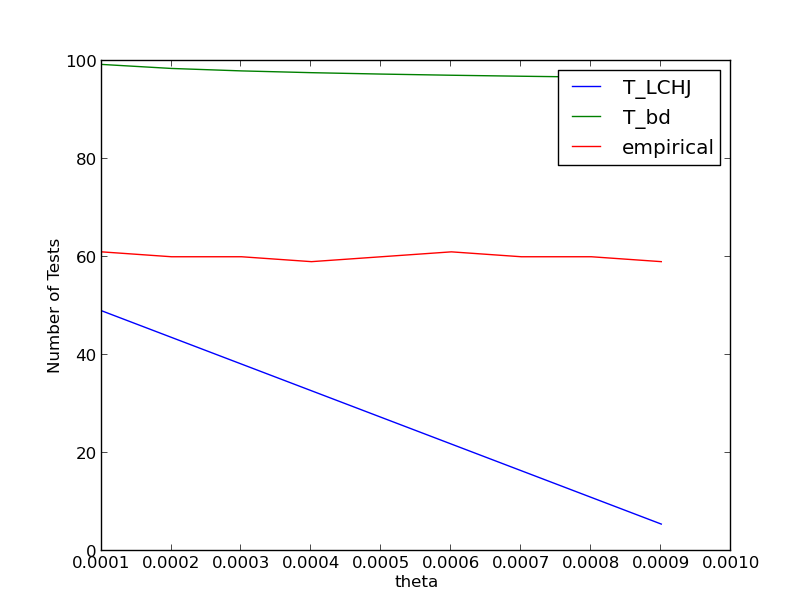
\includegraphics[width=0.5\textwidth]{ubvslb.png}
\caption{Theoretical lower and upper bounds and empirical Test frequencies as functions of \(\theta\)}
\label{ubvslb}
\end{figure}

Note that the Upper bound is not optimal and there still is some room for improvement. Note also that the lower bound degrades with \(\theta_i \). The lower bound (\(T_{LCHJ}\)) was generated according to theorem (\ref{thm:upper}). 

\begin{figure}[h]
\centering
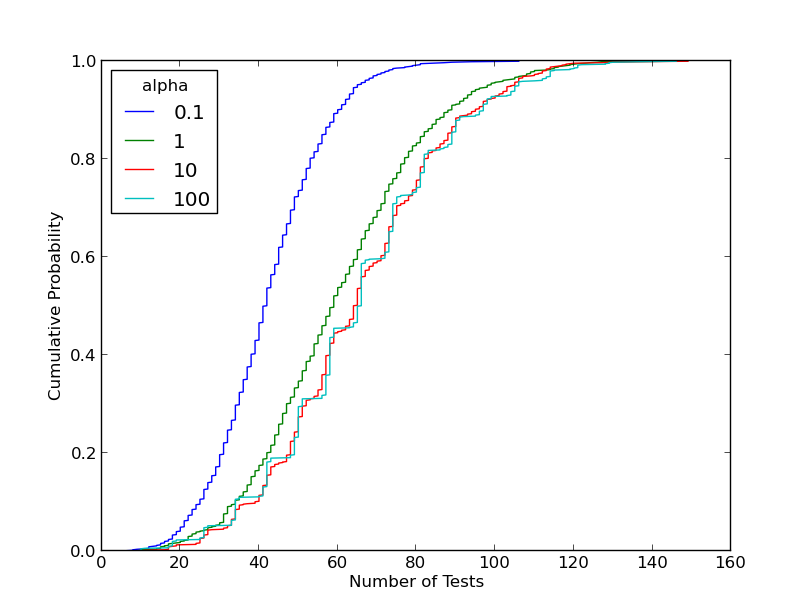
\includegraphics[width=0.5\textwidth]{variousalpha.png}
\caption{Cumulative distribution curves of the modified Hwang algorithm with fixed \(\theta = 0.0001\) and \(\alpha\) varying }
\label{testsvsalpha}
\end{figure}

\begin{figure}[h]
\centering
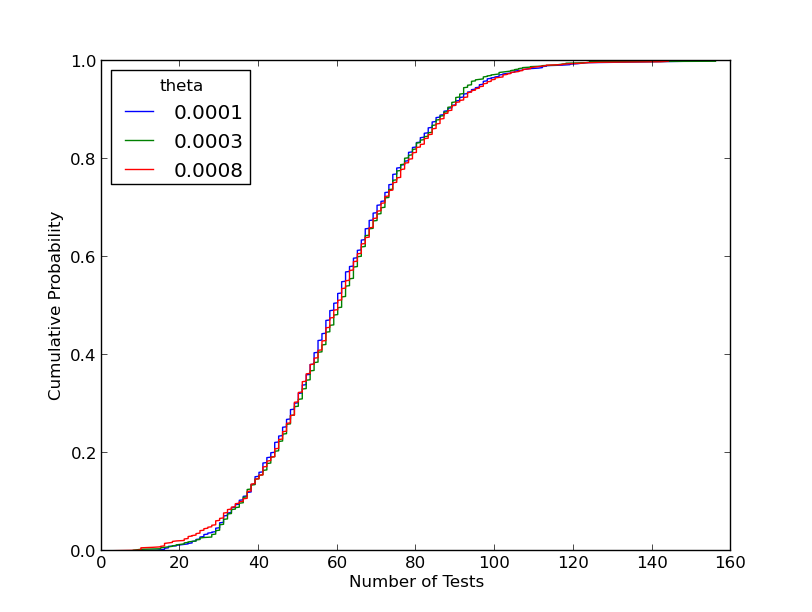
\includegraphics[width=0.5\textwidth]{nicegraphlaminar.png}
\caption{Cumulative distribution curves for fixed \(\alpha = 1\) and varying \(\theta\)}
\label{testsvstheta}
\end{figure}

Figures (\ref{testsvsalpha}) and (\ref{testsvstheta}) show that the performance is relatively insensitive to the cut-off \(\theta\), and more sensitive to the uniformity (or otherwise) of the probability distribution \(\vc{p}\). Heuristically, this is for because distributions which are highly concentrated on a few items algorithms can make substantial savings on the testing budget by testing those highly likely items first (which is captured in the bin structure of the above algorithm). 

The insensitivity to the cutoff \(\theta\) is due to items below \(\theta\) being overwhelmingly unlikely to be defective - which for small \(\theta\) means that few items (relative to the size of the problem) get discarded.

\subsection{Discussion}
%
\dfrac{•}{•}

\section{Sub-Nyquist Sampling techniques}
This section presents some work on sampling methods for wide-band spectrum sensing

\subsubsection{Wideband Modulated Converter} 
The sampling scheme proposed in \cite{Mishali2010} is capable of sampling wideband signals at rates below those predicted by Shannon-Nyquist sampling theory. 

It works by mixing the incoming analogue signal \(x\left(t\right)\) with a mixing function \(p_i\left(t\right)\) aliasing the spectrum. \(x\left(t\right)\) is assumed to be bandlimited and composed of up to \(N_sig\) uncorrelated transmissions (i.e. possible narrowband channels). 

This process is repeated in parallel over \(M\) channels (unrelated to \(N_sig\) so that each band in \(x\) appears in baseband. The mixing functions are required to be periodic, with period \(T_p\). Since \(p_i\) is periodic it has Fourier expansion:

\begin{equation}
p_i\left(t\right) = \sum_{l=-\infty}^{\infty} c_{il} exp{jlt\frac{2\pi}{T_p}}
\end{equation}

The \(c_{il}\) are the Fourier coefficients of the expansion and are defined in the standard manner. The result of the mixing procedure in channel \(i\) is therefore \(xp_i\), with Fourier transform:

\begin{align}
X_{i}\left(f\right) &=& \int_{-\infty}^{\infty} x\left(t\right) p_i\left(t\right) dt
\\ &=& \sum_{l=-\infty}^{\infty} c_{il} X\left(f-lf_p\right)
\end{align}

%\begin{figure*}[h]
%\centering
%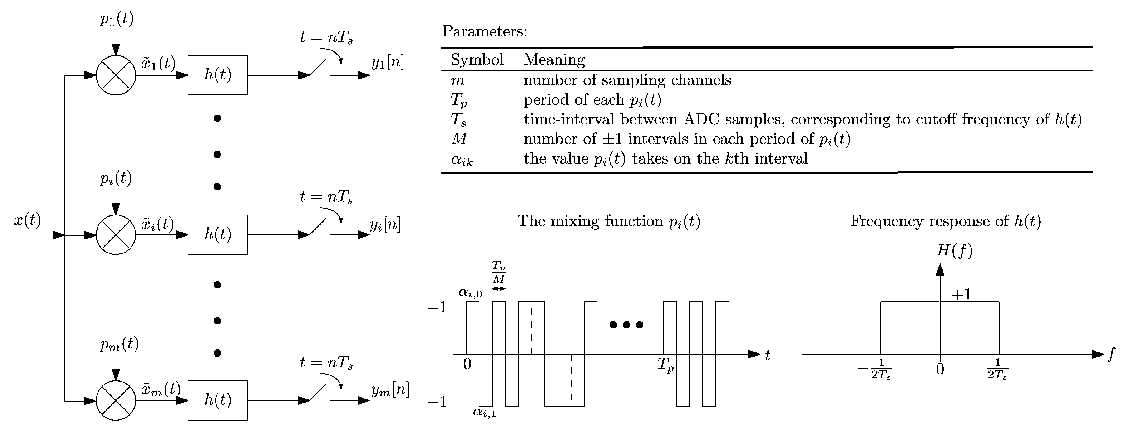
\includegraphics[height = 7 cm, width=\textwidth]{mwc.png}
%\caption{The operation of the Modulated Wideband Converter \cite{Mischali2010}}
%\label{bayesiancs}
%\end{figure*}

(insert the Fourier series for \(p_i\), then exchange the sum and integral). The output of this mixing process then, is a linear combination of shifted copies of \(X\left(f\right)\), with at most \(\lceil f_NYQ/f_p\rceil\) terms since \(X\left(f\right)\) is zero outside it's support (we have assumed this Nyquist frequency exists, even though we never sample at that rate).

Once the mixing process has been completed the signal in each channel is low-pass filtered and sampled at a rate \(f_s \geq f_p\). In the frequency domain this is a ideal rectangle function, so the output of a single channel is:

\begin{equation}
Y_i\left(e^{j 2 \pi f T_s }\right) = \sum_{l = -L_0}^{+L_0}
\end{equation}

since frequencies outside of \([-f_2/2, f_s/2]\) will filtered out. \(L_0\) is the smallest integer number of non-zero contributions in \(X\left(f\right)\) over \([-f_2/2, f_s/2]\) - at most \(\lceil f_NYQ/f_p\rceil\) if we choose \(f_s = f_p\). These relations can be written in matrix form as:

\begin{equation}
\textbf{y} = \textunderscore{\textbf{A}}\textbf{x}
\end{equation}

where \(\textbf{y}\) contains the output of the WMC process, \(\textunderscore{\textbf{A}}\) contains the Fourier coefficients of the mixing functions, and \(\textbf{x}\) is the vector of unknown samples of \(x\left(t\right)\). 


\section{Results and Simulations}
To compare the efficacy of Group Testing and Compressive Sensing, Hwang's algorithm and the algorithm presented in \cite{Aldrouobi} were simulated for a problem size of N=1024 and K=10.  The problem was simulated 100 times and the cumulative distribution found - i.e. after how many tests or measurements were the respective problems solved? This allows the number of tests required by Group Testing to be compared to the number of measurements in Compressive Sensing. Figure \ref{GTvsCS} shows the results:

\begin{figure*}[h]
\centering
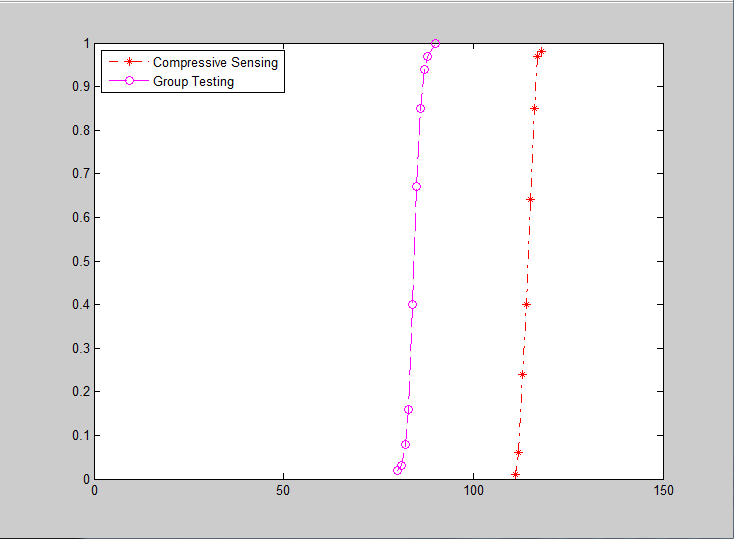
\includegraphics[height = 7 cm]{GTvsCS.png}
\caption{Group Testing vs Compressive Sensing}
\label{GTvsCS} 
\end{figure*}

Note that both the algorithms meet their respective asymptotic bounds (\( \log_2{N \choose K}\) in the case of GT and \(k\log{N}\) for CS). The main point of interest is that Group Testing requires roughly \(\frac{2}{3}\) of the tests required by Compressive Sensing. This is encouraging: despite there being 'less' information - in the sense that the result is a binary number as opposed to a real one -  GT outperforms CS. Intuitively, one would conjecture the opposite - more information should allow you to locate the non-zero components faster. This justifies our interest in the problem, as the performance increase is substantial. 

\section{Further Work and Project Plan}
Both the Compressive Sensing and Group Testing problems have been well studied for the case where there is no prior belief over where the non-zero components of the signal are (or equivalently, which items constitute the defective set). Despite some work being done solving the CS problem in the Bayesian paradigm, the prior distributions used are sparsifying (for example a Laplace prior), and not over the placement of the non-zero components. 

AS such, there is some 'low hanging fruit' to be picked: would using extra information about the likelihood of an item being defective improve the performance of recovery suitably defined? For example, would a Group Testing procedure require fewer tests if there was reason to believe that some subset of items was more likely to be defective. In the coin weighing example discussed above, the input set may contain a coin which is a different colour than the others  - by testing this 'suspicious' coin in the first weighing we could find the counterfeit in a single test (otherwise we would find the counterfeit in at most five tests - one for the suspicious coin, and four following the procedure outlined in the Group Testing section). 

This suggests that using prior information in could significantly reduce the number of tests required to recover the defective set, however if initial tests come back negative the performance of these algorithms could be worsened by using a non-iid distribution. 

To try and characterise this numerical simulations and probabilistic analyses are required. The goal is to design algorithms which have better average case performance than current GT algorithms by incorporating prior beliefs, whilst at the same time do no worse than current performance guarantees. In the example above we'd seek an algorithm that could find the counterfeit coin in a single weighing (by testing the suspicious coin initially), yet could guarantee to find the counterfeit in at most four weighings of the pan balance. 

For the 80 coins, 1 counterfeit discussed above this is probably not possible: adding an extra test which fails before proceeding with the standard approach will always be worse than simply assuming all coins are equally likely to be fake and proceeding accordingly. Do many cases like this exist, and what characterises them? Will testing suspicious items initially always give a hit in performance should those tests fail? 

A few directions into answering these questions are sketched below:

\begin{enumerate}
\item Implicit in the discussion of Hwang's algorithm above is that each item is defective with the same probability \( \frac{K}{N} \). Using prior knowledge over the input set we could test groups of size \(2^\beta\), where \(\beta\) is the empirical expectation of the input set. I.e. modify Hwang's algorithm to test groups in size roughly equal to the (empirical) expectation of the distribution over the input. \textbf{Timeline:} the rest of October 2013. \textbf{Risk: } this is a low risk activity and should take at most a fortnight - the Author has already implemented Hwang's algorithm, so all that needs to be done is to calculate the empiracle mean of the input distribution, and characterise the algorithm in a few cases.

\item Re-formulate the problem in terms of source coding as per \cite{Aldroubi} and represent the items in the input set as a Huffman tree. \textbf{Timeline:} October-December 2013. \textbf{Risk: } medium risk. The Group Testing algorithm will take place over the tree with th groups to test being the branches of the Huffman tree. A bit of the code is ready, however it's not clear how to fit it all together to realise a full solution

\item It has usually been assumed that defective items are independent. Is it possible to relax this assumption, and if so what are the consequences of this for Group Testing algorithms? For example, what happens if defectives occur in clumps? This is a high risk activity, and should take over 6 months to begin to characterise. \textbf{Timeline: }
October 2013-March 2014. \textbf{Risk: } medium risk. Defectives are currently assumed to be independent from each other in the classical Group Testing literature. Motivated by Spectrum Sensing for Cognitive Radios, where available frequencies are not necessarily independent between measurements, we will investigate Group Testing algorithms where the defectives are not independently distributed. Examples include inputs with defective which are pairwise independent, input sets in which the defectives are negatively dependent, and input sets where there is some (random or deterministic) process affecting the distribution of defectives.

\item Some work has been done considering Group Testing as the reverse of Coding \cite{Wadayama2013}, \cite{Sejdinovic2010}, but there is still much to be done. How close is the analogy? Coding theory has a wealth of noise cases - could these be imported into the Group Testing literature, and how useful will they be? \textbf{Timeline: } October 2013 - September 2014. \textbf{Risk: } medium to high risk. A few cases have been explicitly solved (the 'binary-symmetric' and 'erasure' models). Does this analogy extend further, and can techniques from Coding help us in Group Testing. Can we formulate a more general 'Shannon Theory' type theory for Group Testing?

\item To make these models suitable for engineering applications, noisy cases must be considered. \textbf{Timeline: } January - September 2013. \textbf{Risk: } High risk: whereas Group Testing has previously been utilised in Medium Access Control protocol design, it has not been applied to spectrum sensing as of yet. The exact mechanism that can robustly sense spectral opportunities, and make decisions needs careful consideration. Example problems include how should we sample spectra using Group Testing - will a series of wideband pulses over the TVWS band be sufficient, or are is there some other possibility? Once we have these samples, how do then infer spectral opportunities? The work of previous sections (non-iid input distributions, 2D input sets, defectives which are not independent in some way etc) will inform this part of the research. 

\item There currently exist no two-dimensional models of Group Testing in the literature. This is particularly relevant for the problem faced by Cognitive Radios: the radios could represent the measurement point on a geographic grid, and the 'groups' they need to infer are sets of available frequencies. \textbf{Timeline: }  January-April 2014. \textbf{Risk: } High risk: there currently is no work in the literature on 2D group testing. Conjectured methods of solving this problem include factor graph methods from Coding Theory. It's not clear that this is an appropriate method, however.

\end{enumerate}

\bibliography{SummerProject}

\end{document}
